\documentclass[preprint,12pt,authoryear]{elsarticle}

\usepackage[utf8]{inputenc}
\usepackage[T1]{fontenc}
\usepackage{lmodern}
\usepackage{microtype}
\input{glyphtounicode}
\pdfgentounicode=1
\usepackage{amsmath,amssymb,amsfonts,amsthm}
\usepackage{graphicx}
\usepackage{algorithm}
\usepackage{algpseudocode}
\usepackage{booktabs}
\usepackage{multirow}
\usepackage{xcolor}
\usepackage{hyperref}
\usepackage{subcaption}
\usepackage{bm}

\newtheorem{theorem}{Theorem}
\newtheorem{definition}{Definition}

\hypersetup{colorlinks=true,linkcolor=blue,citecolor=blue,urlcolor=blue}

% Custom commands
\newcommand{\R}{\mathbb{R}}
\newcommand{\N}{\mathbb{N}}
\newcommand{\E}{\mathbb{E}}
\newcommand{\Var}{\mathrm{Var}}
\newcommand{\bigO}{\mathcal{O}}
\newcommand{\poly}{\mathrm{poly}}
\newcommand{\polylog}{\mathrm{polylog}}
\newcommand{\tr}{\mathrm{tr}}
\newcommand{\Teff}{T_{\mathrm{eff}}}

\graphicspath{{../../figures/}}

\journal{Neurocomputing}

\begin{document}

\begin{frontmatter}

\title{Memory-Bounded Online Learning under Structured Non-IID Streams: A Proxy-Based Sensitivity Study with Quantum and Classical Baselines}

\author[inst1]{AbdelMoniem Helmy\corref{cor1}}
\ead{abdelmoniem.hafez@cu.edu.eg}
\cortext[cor1]{Corresponding author.}

\author[inst2]{Muhammad Mahmoud}
\ead{m.mahmoud@mau.edu.eg}

\affiliation[inst1]{organization={Department of Information Systems and Technology, Faculty of Graduate Studies for Statistical Research, Cairo University},
  city={Cairo},
  country={Egypt}}

\affiliation[inst2]{organization={Information Systems Department, Faculty of Computers and Artificial Intelligence, Matrouh University},
  country={Egypt}}

\begin{abstract}
Quantum oracle sketching achieves exponential memory advantages over classical streaming for tasks such as classification and dimension reduction \citep{zhao2026exponential}, and its theoretical framework extends to non\nobreakdash-IID data; however, the behaviour of these robustness guarantees under structured correlation patterns relevant to practice remains unexplored, and no prior work has systematically mapped how specific correlation families---Markov dependence, seasonal drift, burst repetition, long-range dependence---affect the estimated performance of quantum oracle sketching relative to classical streaming baselines. To close this gap we introduce operational correlation proxies---a refreshing time $\tau$ and a repetition number $r$---inspired by the correlated-data framework of Zhao et al.\ (2026) and use them to conduct a proxy-based computational study across five structured synthetic non\nobreakdash-IID regimes. For each regime we specify analytic proxy expressions for $\tau$ and $r$, compare them against 10-seed empirical measurements on generated streams, run three classical memory-bounded streaming baselines (online SGD, averaged SGD, and a Count-Min-style hash classifier), and compute heuristic quantum performance proxies, reporting all stochastic results as 10-seed means with 95\% confidence bands and paired Wilcoxon significance tests for the main comparisons. When the empirical refreshing time is used the proxy model predicts a favourable region under mild-to-moderate correlation, while stronger correlation reduces the proxy-estimated separation; where analytic proxies overestimate the empirical refreshing time the gap reaches up to roughly $125\times$ for long-memory data, indicating that tighter family-specific characterisations could substantially enlarge the predicted advantage region, whereas in the IID and burst regimes the empirical values instead exceed the analytic proxy, reflecting finite-sample autocorrelation fluctuations and, for burst, forward-window counting effects at the chosen window length. A sensitivity landscape in $(\tau, r)$ space visualises contours of the quantum accuracy proxy across correlation conditions and serves as the paper's central operational artefact. This is a modelling study using heuristic proxies primarily on synthetic data, augmented with two real-stream case studies (NYC Taxi and Machine Temperature, both from the Numenta Anomaly Benchmark) reported with imbalance-aware balanced accuracy and $F_1$ alongside accuracy, and four sensitivity ablations; it does not implement or simulate any quantum algorithm and does not validate the full Zhao et al.\ theory, and broader real-stream validation across financial, network-traffic, and additional sensor domains remains future work.
\end{abstract}

\begin{keyword}
online learning \sep streaming classifiers \sep non\nobreakdash-IID data \sep concept drift \sep correlation sensitivity analysis \sep memory-bounded learning \sep quantum oracle sketching
\end{keyword}

\end{frontmatter}

%=====================================================================
\section{Introduction}
\label{sec:intro}
%=====================================================================

The exponential growth of data-intensive applications in domains such as sensor networks, financial markets, climate monitoring, and telecommunications has created an urgent need for streaming algorithms that process data on the fly with severely constrained memory \citep{muthukrishnan2005data}. Classical streaming algorithms---including sketching methods, online learners, and sliding-window estimators---offer practical solutions but face fundamental memory--accuracy tradeoffs rooted in information-theoretic lower bounds \citep{alon1999space}. A further complication is that real-world streams are rarely IID: Internet traffic exhibits long-range dependence and self-similarity \citep{leland1994ethernet, willinger1997selfsimilarity}, and streaming-ML systems must contend with concept drift and non-stationary input distributions \citep{gama2014driftsurvey, arora2024driftreview, su2024elasticonline, yan2024bidynamic}.

Recent work by \citet{zhao2026exponential} shows that quantum oracle sketching achieves exponential quantum advantages for classification and dimension reduction on massive classical data, using a polylogarithmic-size quantum computer ($\bigO(n)$ qubits for $n = \log_2 N$). For several concrete problems the classical memory requirement scales polynomially in $N = 2^n$, yielding an exponential gap; the classical hardness results are task-specific \citep{harrow2009hhl, havlicek2019qkernels, schuld2021encoding, biamonte2017qml}. The broader quantum ML landscape includes variational algorithms \citep{cerezo2021variational}, NISQ-era perspectives \citep{preskill2018nisq}, quantum learning theory \citep{schuld2018supervised}, and classical shadow tomography \citep{huang2020shadows}.

A particularly notable feature of this framework is its treatment of non\nobreakdash-IID data. \citet{zhao2026exponential} extend their analysis to correlated, non\nobreakdash-IID data via a structured data-generation model in which the quantum sample complexity increases with the degree of data correlation. However, the practical implications of this robustness under structured, real-world correlation patterns remain unexplored.

Four questions motivate our study: (RQ1) How tight are the generic robustness guarantees for specific structured families? (RQ2) How informative are $\tau$ and $r$ as accuracy predictors? (RQ3) Under what correlation conditions does the proxy-estimated favourable separation persist, degrade, or potentially improve? (RQ4) How do empirically measured $(\tau, r)$ relate to the analytic proxy predictions?

\paragraph{Scope} The scope is a \textbf{proxy-based computational sensitivity study of memory-bounded online learning under structured non\nobreakdash-IID streams}: operational correlation proxies inspired by the Zhao et al.\ framework are used to map where proxy-estimated performance is most favourable under the modelling assumptions across structured synthetic non\nobreakdash-IID conditions, with a two\nobreakdash-dataset real-stream sanity check (Section~\ref{sec:real_stream}). Quantum performance curves are heuristic proxies and no quantum algorithm is implemented; circuit simulation, primary-source theorem reproduction, and broader real-stream validation remain explicit follow-on targets (Section~\ref{sec:future_work}).

We study five non\nobreakdash-IID regimes (IID, Markov switching, seasonal drift, burst repetition, long-range dependence), specifying analytic proxy expressions for $\tau$ and $r$, measuring their empirical counterparts on generated streams, comparing three classical baselines, and mapping results onto a $(\tau, r)$ sensitivity landscape with 10-seed means, 95\% CI bands, and paired Wilcoxon tests.

Our principal contributions are:

\begin{enumerate}
    \item \textbf{Operational correlation proxies} for five structured non\nobreakdash-IID regimes, explicitly labeled as engineering approximations rather than theorems.

    \item \textbf{Empirical-vs-proxy gap analysis} showing that, where analytic proxies overestimate empirical refreshing time, the gap ranges from roughly $8\times$ (Markov) to $125\times$ (long-memory); in the IID and burst regimes the empirical values instead exceed the analytic proxy, reflecting finite\nobreakdash-sample autocorrelation fluctuations and, for burst, forward\nobreakdash-window counting effects at the chosen window length. These directional gaps indicate where tighter family-specific characterisations are most needed.

    \item \textbf{A $(\tau, r)$ sensitivity landscape} that maps the quantum accuracy proxy as a function of correlation parameters, identifying regions where the proxy accuracy is highest and which can serve as a diagnostic map for proxy-side sensitivity analysis.

    \item \textbf{Regime-dependent robustness trends:} the proxy model suggests a favourable region under mild to moderate correlation that narrows predictably as correlation strengthens.
\end{enumerate}

Sections~\ref{sec:related}--\ref{sec:prelim} review related work and introduce the proxy model; Section~\ref{sec:theory} specifies the correlation proxies; Section~\ref{sec:experiments} describes the experimental setup; Section~\ref{sec:results} presents nine experiments (seven on synthetic streams, a two\nobreakdash-dataset real-stream sanity check, and an ablation suite); Section~\ref{sec:discussion} discusses implications and limitations; Section~\ref{sec:conclusion} concludes.


%=====================================================================
\section{Related Work}
\label{sec:related}
%=====================================================================

\subsection{Classical Streaming Algorithms}

Classical data streaming has been studied extensively since the seminal work of \citet{alon1999space} on frequency moments \citep{muthukrishnan2005data}. Key developments relevant to this paper include the Count-Min Sketch of \citet{cormode2005improved} for frequency estimation, the Frequent Directions algorithm of \citet{ghashami2016frequent} for streaming low-rank approximation, and the sketching-as-linear-algebra framework of \citet{woodruff2014sketching}. On the learning side, \citet{shalev2012online} provides the standard reference for online convex optimisation; \citet{polyak1992averaging} introduced Polyak--Ruppert averaging, which we use as a second classical baseline; and \citet{weinberger2009featurehashing} established the feature-hashing technique underlying our bounded-memory classifier.

The behaviour of streaming algorithms under structured temporal correlation has received comparatively less attention. Concept drift is surveyed by \citet{gama2014driftsurvey} and \citet{ditzler2015nonstationary}; ADWIN \citep{bifet2007adwin} is the canonical adaptive-window solution. Broader online-learning treatments appear in MOA \citep{bifet2010moa}, \citet{hoi2021online}, and \citet{gama2010knowledge}; the most recent systematic drift review is \citet{arora2024driftreview}; adaptive random forests \citep{gomes2017adaptiverf} serve as the drift-aware classical reference. Recent work on non-stationary streaming includes elastic online deep-learning pipelines \citep{su2024elasticonline}, bi-dynamic-distribution learning \citep{yan2024bidynamic}, and feature-based drift analyses \citep{hinder2024featuredrift}. Non-stationary online optimisation is analysed in \citet{besbes2015non} and \citet{ben2010agnostic}; Count-Min refinements appear in \citet{benmazziane2022countmin} and \citet{cormode2011synopses}; foundational self-similarity measurements are in \citet{park2000selfsimilar}.

\subsection{Quantum Advantages for Data Processing}

Quantum algorithms for data processing include quantum SVMs \citep{rebentrost2014quantum}, quantum PCA \citep{lloyd2014quantum}, the quantum singular value transformation \citep{gilyen2019qsvt} with block-encoding subroutines \citep{chakraborty2019blockencodings}. Critical perspectives on access-model dependencies appear in \citet{aaronson2015readthefineprint} and \citet{tang2019quantum}; qRAM feasibility is discussed in \citet{giovannetti2008quantum}; surveys include \citet{chen2024qmlsurvey} and \citet{schuld2018supervised}. Quantum advantages depend critically on data structure and access \citep{huang2021powerofdata}; an experimental demonstration of exponential advantage appears in \citet{huang2022experiments}. On quantum streaming: \citet{kallaugher2021streaming} established the first exponential quantum-classical space separation for a natural streaming problem; \citet{kallaugher2025designquantum} provided a black-box quantum-sketch construction for classical algorithm designers. The quantum oracle sketching framework of \citet{zhao2026exponential} avoids qRAM entirely and supports exponential separations for classification and dimension-reduction tasks.

\subsection{Non-IID Data in Quantum Computing}

\citet{arunachalam2018optimal} study quantum sample complexity under the IID PAC assumption. The quantum oracle sketching framework \citep{zhao2026exponential} is, to our knowledge, the first to address noisy, correlated, and time-varying classical data in a quantum streaming setting. We introduce operational proxies inspired by their correlated-data discussion across five structured regimes; the Markov mixing time follows product-chain results \citep{levin2017mixing} and the long-memory statistics follow fGn theory \citep{mandelbrot1968fbm, beran1994statistics}.


%=====================================================================
\section{Preliminaries}
\label{sec:prelim}
%=====================================================================

\subsection{Quantum Oracle Sketching}

\citet{zhao2026exponential} show that a polylogarithmic-size quantum computer ($\bigO(n)$ qubits for $n$-dimensional data, $N = 2^n$) can perform classification and dimension reduction on massive classical data by processing random samples on the fly via quantum oracle sketching; Boolean function learning is one concrete instantiation. For several concrete tasks, the classical memory requirement scales polynomially in $N$, yielding an exponential memory gap. Their correlated-data extension uses a structured data-generation model that accounts for temporal dependence; we adopt the terms \emph{refreshing time} (decorrelation scale) and \emph{repetition number} (expected duplication) as our operational labels for the key correlation parameters, noting that our definitions (Section~\ref{sec:heuristic_model}) are inspired by but not necessarily identical to the exact quantities in their framework. Classical hardness results are task-specific, not a universal lower bound.

\subsection{Heuristic Effective-Sample Model}
\label{sec:heuristic_model}

\textbf{Proxy status.} The quantities $\tau$ and $r$ defined below are \emph{paper-defined operational proxies} motivated by, but not formally equivalent to, the correlation parameters discussed in \citet{zhao2026exponential}; equivalence proofs are follow-on work. We introduce a simplified effective-sample proxy that adapts the qualitative structure of the correlated-data discussion in \citet{zhao2026exponential} into a tractable form for computational exploration across diverse correlation families. The choice $C{=}2$, $\delta{=}0.05$ in Eq.~\eqref{eq:oracle_error} rescales accuracy contours uniformly without deforming the qualitative regime ordering: changing $C$ or $\delta$ shifts every contour along the hyperbolic family $\tau r \propto (C^2 \log(1/\delta))^{-1}$, preserving the relative ranking of all regimes. Practitioners interpreting the landscape quantitatively should treat absolute contour values as indicative rather than universal.

\begin{definition}[Refreshing Time -- operational proxy]
We define the \emph{operational refreshing time} $\tau$ of a data stream as the smallest lag at which the normalized autocorrelation drops below $1/e$. This is an empirically measurable quantity that serves as a proxy for the decorrelation rate of the stream.
\end{definition}

\begin{definition}[Repetition Number -- operational proxy]
We define the \emph{operational repetition number} $r$ as $1$ plus the expected number of \emph{exact duplicate} copies of each sample within a forward window of length $W$. Throughout this paper we use $W = 20$ in the empirical estimator; this is the definition that Fig.~\ref{fig:corr_char}(b) reports and matches the analytic family-level $r$ in units.
\end{definition}

We model the effective independent sample count as:
\begin{equation}
\Teff = T / (\tau \cdot r),
\label{eq:teff}
\end{equation}
and use the following heuristic oracle error proxy:
\begin{equation}
\epsilon \leq C \sqrt{\frac{n \log(1/\delta)}{\Teff}},
\label{eq:oracle_error}
\end{equation}
where $C = 2$ and $\delta = 0.05$ throughout our experiments. Under IID data, $\tau = 1$ and $r = 1$, recovering the standard scaling $\epsilon \sim \sqrt{n/T}$.

For the quantum memory requirement, \citet{zhao2026exponential} prove that $\bigO(n)$ qubits suffice for oracle construction. On the classical side, they also prove task-specific lower bounds that scale polynomially in $N = 2^n$ for certain problems (e.g., regimes where the target function forces classical algorithms to store a polynomial fraction of the truth table). Throughout this paper we use $\Omega(\sqrt{N})$ as a \emph{representative, worst-case} classical memory reference point; it is the bound that motivates the exponential separation in their analysis, \emph{not} an empirically witnessed floor for the online-gradient classical learners studied here. For the 10-dimensional linear classification task used in our experiments, the classical learner is in fact sample-limited rather than memory-limited once $M$ exceeds a small threshold (Section~\ref{sec:acc_vs_memory}). The $\Omega(\sqrt{N})$ curve in our figures therefore illustrates the worst-case asymptotic separation, not the empirical gap on the specific task studied.

The heuristic classification accuracy proxy used in our experiments is:
\begin{equation}
\mathrm{acc\_proxy} = \max\!\left(0.5,\; 1 - \epsilon^2\right),
\label{eq:acc_proxy}
\end{equation}
where the floor of $0.5$ represents the random-guess baseline for binary classification. When $\epsilon^2 > 0.5$ (as occurs in the long-memory regime), the proxy saturates at $0.5$, reflecting that the model predicts no useful signal. This is an engineering surrogate that translates oracle approximation quality into a classification metric for visualization.


%=====================================================================
\section{Correlation Proxies for Specific Data Families}
\label{sec:theory}
%=====================================================================

We specify heuristic expressions for the operational $\tau$ and $r$ under five concrete correlation regimes. Each is an engineering proxy motivated by the autocorrelation or mixing structure of the regime; tighter proofs of equivalence to the correlation parameters in Zhao et al.\ are follow-on work.

\subsection{Regime 1: IID Baseline}

Under IID sampling from a uniform distribution over $\{0,1\}^n$:
\begin{equation}
    \tau_{\text{IID}} = 1, \qquad r_{\text{IID}} = 1, \qquad \Teff = T.
\end{equation}
This serves as the reference against which all other regimes are compared.

\subsection{Regime 2: Markov Switching}

Consider a Markov chain on $\{0,1\}^n$ where each bit flips independently with probability $(1 - \rho)/2$ at each step, for correlation parameter $\rho \in [0, 1)$. The stationary distribution is uniform.

The mixing time of this product chain is $\Theta(n \log n / (1 - \rho))$. We use the simplified engineering proxy:
\begin{equation}
    \tau_{\text{Markov}}(\rho, n) \approx \frac{n}{1 - \rho},
    \label{eq:tau_markov}
\end{equation}
which preserves the dominant divergence as $\rho \to 1$ while suppressing logarithmic and model-specific constants. \emph{Provenance:} the $1/(1{-}\rho)$ scaling is theory-motivated (mixing-time asymptotics); the omission of the $\log n$ factor is an engineering simplification; the equivalence to the correlation parameters in \citet{zhao2026exponential} is unvalidated. Since samples from a Markov chain are not repeated exactly, $r_{\text{Markov}} = 1$, giving $\Teff \approx T(1{-}\rho)/n$.

\subsection{Regime 3: Seasonal Drift}

Consider a stream where bit $i$ at time $t$ is drawn as Bernoulli with probability $p_i(t) = \tfrac{1}{2} + \alpha \sin(2\pi t/P + \phi_i)$, where $P$ is the period, $\alpha \in (0, 0.5)$ is the drift strength, and $\phi_i$ are fixed phase offsets.

The seasonal regime is \emph{distributional drift}: samples at distinct times are conditionally independent given $t$, making this non\nobreakdash-IID only in the weak sense of non-stationary marginals. It is included because both the quantum oracle construction and classical learners are affected by marginal drift, and because it is a common practical stream pattern.

We propose the decorrelation proxy:
\begin{equation}
    \tau_{\text{Seasonal}}(P, \alpha) = \max(1,\; P \cdot \alpha),
    \label{eq:tau_seasonal}
\end{equation}
lower-bounded by 1 to ensure $\tau \geq \tau_{\text{IID}}$ in all cases. \emph{Provenance:} the product $P\alpha$ captures the intuition that decorrelation scales with both period and drift strength; the functional form $\max(1, P\alpha)$ is an engineering convenience with no formal derivation. Since the distribution changes continuously, $r_{\text{Seasonal}} = 1$.

\subsection{Regime 4: Burst Repetition}

In the burst model, at each step, with probability $p_b$ the previous sample is exactly repeated for an additional $L$ consecutive copies (i.e., the burst contributes $L$ duplicate observations). The expected number of observations per effective fresh sample is therefore:
\begin{equation}
    r_{\text{Burst}}(L, p_b) = 1 + p_b \cdot L.
    \label{eq:r_burst}
\end{equation}
\emph{Provenance:} the formula follows directly from the model definition (theory\nobreakdash-motivated); the assumption that duplicates contribute no new information is exact for our synthetic generator but would require validation on real burst-prone streams. Since bursts do not affect the mixing of fresh samples, $\tau_{\text{Burst}} = 1$, giving $\Teff = T/(1 + p_b L)$.

\subsection{Regime 5: Long-Range Dependence}

For streams driven by fractional Gaussian noise (fGn) with Hurst parameter $H \in (0.5, 1)$, the autocorrelation of the \emph{underlying Gaussian process} decays as a power law, and integrated autocorrelation grows as $T^{2H-1}$. We adopt as our proxy the horizon-dependent correlation penalty:
\begin{equation}
    \tau_{\text{LRD}}(H, T) = T^{2H-1},
    \label{eq:tau_lrd}
\end{equation}
yielding $\Teff = T^{2(1-H)}$.

\paragraph{Proxy status} Equation~\eqref{eq:tau_lrd} is an \emph{upper-bound proxy}. In our construction the stream is a \emph{binarized} fGn (each bit is a thresholded fGn path); binarization converts Gaussian autocorrelation $\gamma(k)$ into binary autocorrelation $(2/\pi)\arcsin(\gamma(k))$, which is strictly smaller in absolute value. The effective decorrelation of the binary stream is therefore \emph{faster} than Eq.~\eqref{eq:tau_lrd} suggests, so the proxy is conservative. Deriving a tighter proxy that accounts for the arcsine transformation is deferred to future work. Unlike the other regimes, this proxy depends on the stream length $T$, reflecting the property that the underlying driving process has no finite decorrelation time.

\subsection{Summary}

Table~\ref{tab:bounds} summarizes the proxy parameters and heuristic MSE proxy values for each regime, computed from the single master formula $\epsilon^2 = \min(1,\, C^2 n \log(1/\delta) / \Teff)$ with $C = 2$ and $\delta = 0.05$.

\begin{table}[t]
\centering
\caption{Summary of heuristic correlation proxies and MSE proxy values ($\epsilon^2$) for each regime, with $T = 10{,}000$, $n = 10$, $C = 2$, and $\delta = 0.05$. The factor $\kappa = C^2 \log(1/\delta) \approx 12$.}
\label{tab:bounds}
\begin{tabular}{@{}lcccc@{}}
\toprule
Regime & $\tau$ & $r$ & $\Teff$ & MSE proxy $\min(1, \kappa n / \Teff)$ \\
\midrule
IID & 1 & 1 & 10{,}000 & 0.012 \\
Markov ($\rho{=}0.7$) & $n/(1{-}\rho) \approx 33$ & 1 & $\approx 300$ & 0.40 \\
Seasonal ($P{=}100, \alpha{=}0.3$) & $\max(1, P\alpha) = 30$ & 1 & $\approx 333$ & 0.36 \\
Burst ($L{=}10, p{=}0.3$) & 1 & $1{+}pL = 4$ & 2{,}500 & 0.048 \\
Long-memory ($H{=}0.8$) & $T^{2H{-}1} \approx 251$ & 1 & $\approx 40$ & 1.0 (saturated) \\
\bottomrule
\end{tabular}

\end{table}


%=====================================================================
\section{Experimental Framework}
\label{sec:experiments}
%=====================================================================

Throughout this section, the comparison is between (1)~empirical bounded-memory classical learners evaluated on a simple linear classification task, and (2)~a theory-inspired heuristic proxy for quantum oracle sketching performance; the empirical classical baselines are not the hard problem instances from \citet{zhao2026exponential}.

\subsection{Data Generation and Diagnostics}

Data streams over $\{0,1\}^n$ with $n = 10$ ($N = 1{,}024$) and $T \leq 20{,}000$. Target task: binary classification with random linear separator $f(x) = \mathbf{1}[\langle x - \tfrac{1}{2}\mathbf{1}, w \rangle > 0]$, $w \in \R^n$ fixed. Parameter values follow Section~\ref{sec:theory}: IID (uniform), Markov ($\rho = 0.7$), Seasonal ($P = 100$, $\alpha = 0.3$), Burst ($L = 10$, $p_b = 0.3$), Long-memory ($H = 0.8$).

Empirical diagnostics: $\tau$ is the smallest lag where normalized autocorrelation (averaged over bits) drops below $1/e$; $r$ is $1$ plus the mean exact-duplicate count in a $W = 20$ forward window.

\subsection{Classical Baselines}

Three memory-bounded streaming classifiers cover the key axes:
\begin{itemize}
    \item \textbf{Online SGD}: logistic regression with feature hashing \citep{weinberger2009featurehashing, shalev2012online}; memory $\bigO(M)$.
    \item \textbf{Averaged SGD}: Polyak--Ruppert running average $\bar{w}_t = \frac{1}{t}\sum_s w_s$ \citep{polyak1992averaging}; lower variance than plain SGD.
    \item \textbf{Count-Min hash classifier}: Count-Min Sketch \citep{cormode2005improved} as a label-averaging lookup table; serves as a collision-limited non-gradient reference (near-chance for $M \ll N$).
\end{itemize}
Memory budgets range from $M = 8$ to $M = 256$.

\subsection{Quantum Performance Proxies}
\label{sec:quantum_proxies}

Rather than simulating quantum circuits (which would require exponential classical resources at meaningful scale), we compute proxy quantities from the effective-sample model of Section~\ref{sec:heuristic_model}:
\begin{itemize}
    \item Oracle MSE proxy: $\epsilon^2 = C^2 n \log(1/\delta) / \Teff$, with $C = 2$, $\delta = 0.05$.
    \item Classification accuracy proxy: $\mathrm{acc\_proxy} = \max(0.5,\; 1 - \epsilon^2)$ (Eq.~\ref{eq:acc_proxy}).
    \item Quantum memory: $\bigO(n)$ qubits \citep{zhao2026exponential}.
\end{itemize}

\paragraph{Justification of proxy constants and forms} Three design choices in the proxy expressions warrant explicit discussion.
(i) The constant $C = 2$ in $\epsilon^2 = C^2 n \log(1/\delta) / \Teff$ is a conservative scaling factor consistent with concentration-inequality constants in the quantum oracle sketching literature; alternative values $C \in \{1, 1.5, 2.5\}$ scale the proxy curve uniformly and preserve all relative orderings between regimes.
(ii) The confidence parameter $\delta = 0.05$ matches the 95\% reporting convention used throughout the paper; a $10\times$ change in $\delta$ shifts $\log(1/\delta)$ by a factor of only ${\approx}1.5$, which is small relative to the cross-regime differences in $\Teff$.
(iii) The seasonal proxy $\tau = \max(1, P\alpha)$ is an engineering convenience encoding that periodic streams effectively reset every ${\sim}P\alpha$ samples; the long-memory proxy uses an arcsine correction following \citet{beran1994statistics} to account for binarisation, and is acknowledged as conservative. Section~\ref{sec:ablations} reports an explicit sensitivity analysis under four alternative $\tau$ estimators and three target functions, and shows that the qualitative regime ordering is preserved.

\paragraph{Measured vs.\ proxy} \textbf{Empirically measured} (10 seeds, 95\% CI): classical accuracy, $\tau_{\text{emp}}$, $r_{\text{emp}}$. \textbf{Proxy-estimated} (deterministic): $\Teff = T/(\tau r)$, $\epsilon^2 = \min(1, \kappa n/\Teff)$ with $\kappa \approx 12$, $\mathrm{acc\_proxy} = \max(0.5, 1-\epsilon^2)$. All figures clearly distinguish the two categories; deterministic landscapes (Fig.~\ref{fig:landscape}) have no seed dependency.

\paragraph{Reproducibility parameters} Table~\ref{tab:repro} consolidates all fixed experimental constants for independent reimplementation.

\begin{table}[t]
\centering
\caption{Reproducibility summary: fixed experimental parameters.}
\label{tab:repro}
\begin{tabular}{@{}ll@{}}
\toprule
Parameter & Value / method \\
\midrule
Seeds per experiment & 10 (indices 0--9) \\
Forward window $W$ & 20 \\
Proxy constants & $C = 2$, $\delta = 0.05$, $\kappa = C^2 \log(1/\delta) \approx 12$ \\
$\tau_{\text{emp}}$ estimator & smallest lag $k$ where mean bit-wise autocorrelation $< 1/e$ \\
$r_{\text{emp}}$ estimator & $1 +$ mean exact-duplicate count in $W$-forward window \\
Wilcoxon pairing & each seed's classical accuracy paired with same-seed proxy value \\
Stochastic quantities & classical accuracy, $\tau_{\text{emp}}$, $r_{\text{emp}}$ (10-seed, 95\% CI) \\
Deterministic quantities & $\Teff$, $\epsilon^2$, $\mathrm{acc\_proxy}$, $(\tau,r)$ landscape \\
\bottomrule
\end{tabular}
\end{table}


%=====================================================================
\section{Results and Discussion}
\label{sec:results}
%=====================================================================

We now present nine experiments. Experiments~1--7 are visualisation experiments on the synthetic non\nobreakdash-IID regimes, each accompanied by multi-seed classical baselines on the same streams: Experiments~1--2 compare accuracy trajectories; Experiment~3 presents the analytic $(\tau, r)$ sensitivity landscape; Experiment~4 contrasts empirical and analytic correlation parameters; Experiment~5 sweeps Markov correlation strength; Experiment~6 examines dimension scaling; Experiment~7 shows rolling-accuracy dynamics over time. Experiment~8 is a real-stream sanity check on two NAB datasets (Section~\ref{sec:real_stream}); Experiment~9 is a sensitivity-ablation suite (Section~\ref{sec:ablations}).

\subsection{Experiment 1: Classification Accuracy vs.\ Sample Count}

\begin{figure}[t]
    \centering
    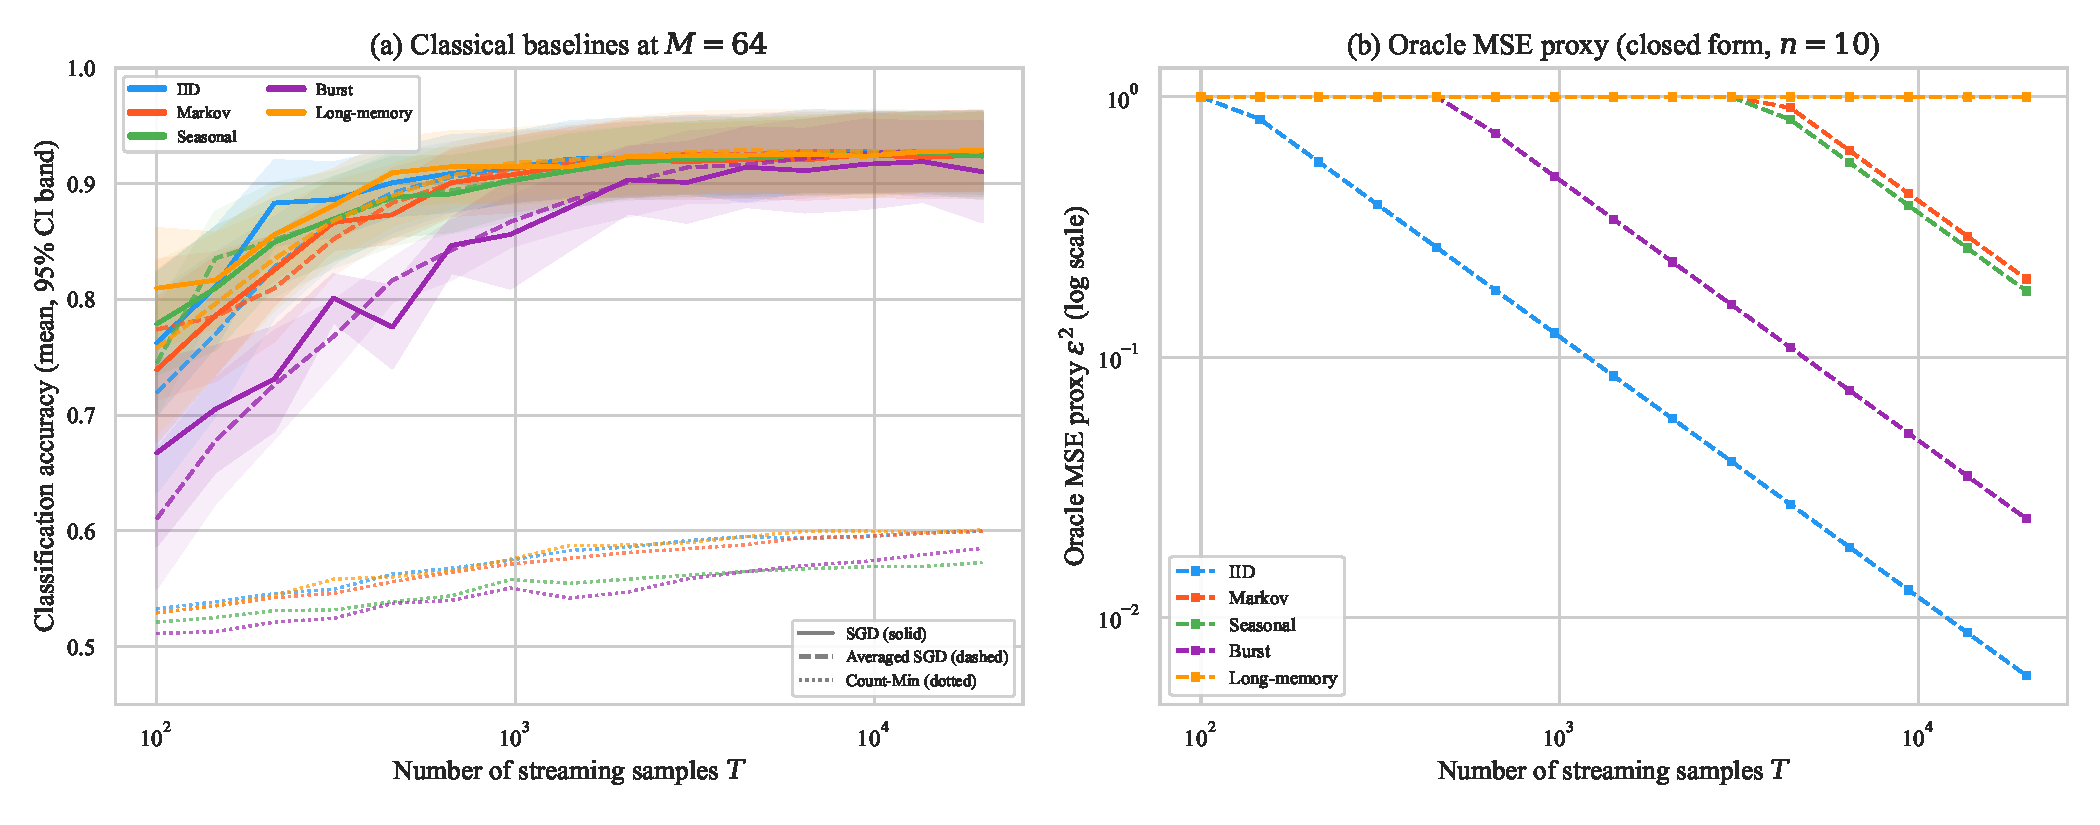
\includegraphics[width=\textwidth]{fig1_accuracy_vs_samples.pdf}
    \caption{Classification accuracy and quantum proxy error vs.\ stream length $T$ (10-seed mean, 95\% CI bands). \textbf{(a)} Three classical baselines at $M = 64$: online SGD (solid), averaged SGD (dashed), Count-Min (dotted). \textbf{(b)} Quantum oracle MSE proxy $\epsilon^2$ ($n = 10$ qubits), log-log scale.}
    \label{fig:accuracy}
\end{figure}

Figure~\ref{fig:accuracy} shows that all classical baselines converge to $0.88$--$0.92$ accuracy with narrow CI bands. Averaged SGD (Polyak--Ruppert, \citealp{polyak1992averaging}) produces smoother trajectories, particularly in the burst regime; Count-Min saturates near $0.55$--$0.60$ due to hash collisions at $M \ll N$. The MSE proxy (Panel b) decays as $1/\Teff$: IID and burst show fast decay; for Markov, seasonal, and long-memory, analytic $\tau$ inflates $\epsilon^2$ enough that the accuracy proxy falls below classical (Section~\ref{sec:correlation_char} quantifies this).

\subsection{Experiment 2: Classical Accuracy vs.\ Memory Budget}
\label{sec:acc_vs_memory}

\begin{figure}[t]
    \centering
    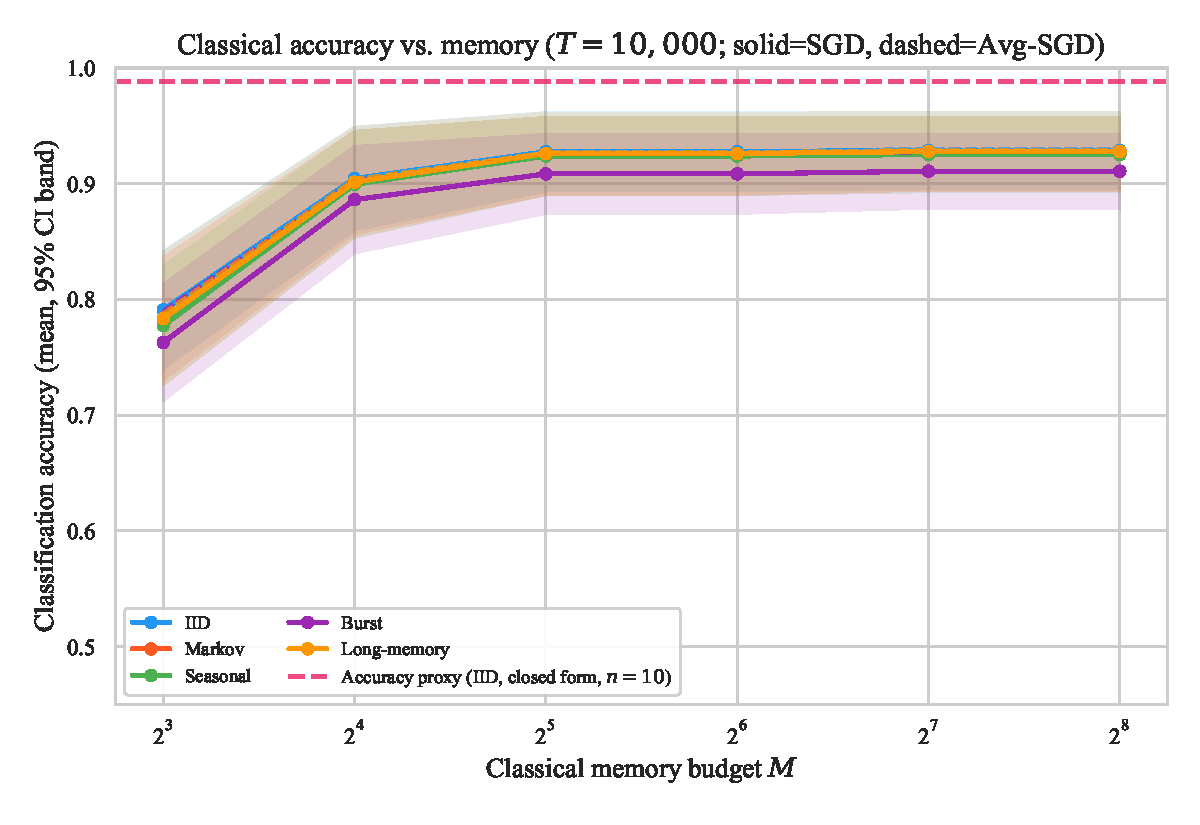
\includegraphics[width=0.7\textwidth]{fig2_accuracy_vs_memory.pdf}
    \caption{Classical online SGD accuracy vs.\ memory $M$ ($T = 10{,}000$) compared with the quantum IID proxy (dashed). Classical accuracy saturates at $M \geq 16$; under the IID modelling assumptions, the IID proxy lies above the empirical classical curves on this task.}
    \label{fig:accuracy_memory}
\end{figure}

Figure~\ref{fig:accuracy_memory} shows that classical accuracy saturates at $M \geq 16$, confirming that the SGD learner is sample-limited rather than memory-limited at this scale. Under the IID modelling assumptions, the IID proxy curve (${\sim}0.99$) lies above the empirical classical curves on this task---a proxy-side ordering, not an implemented algorithmic comparison; the $\Omega(\sqrt{N})$ memory reference is a task-specific worst-case floor \citep{zhao2026exponential}.

\subsection{Experiment 3: Sensitivity Landscape in $(\tau, r)$ Space}
\label{sec:landscape}

\begin{figure}[t]
    \centering
    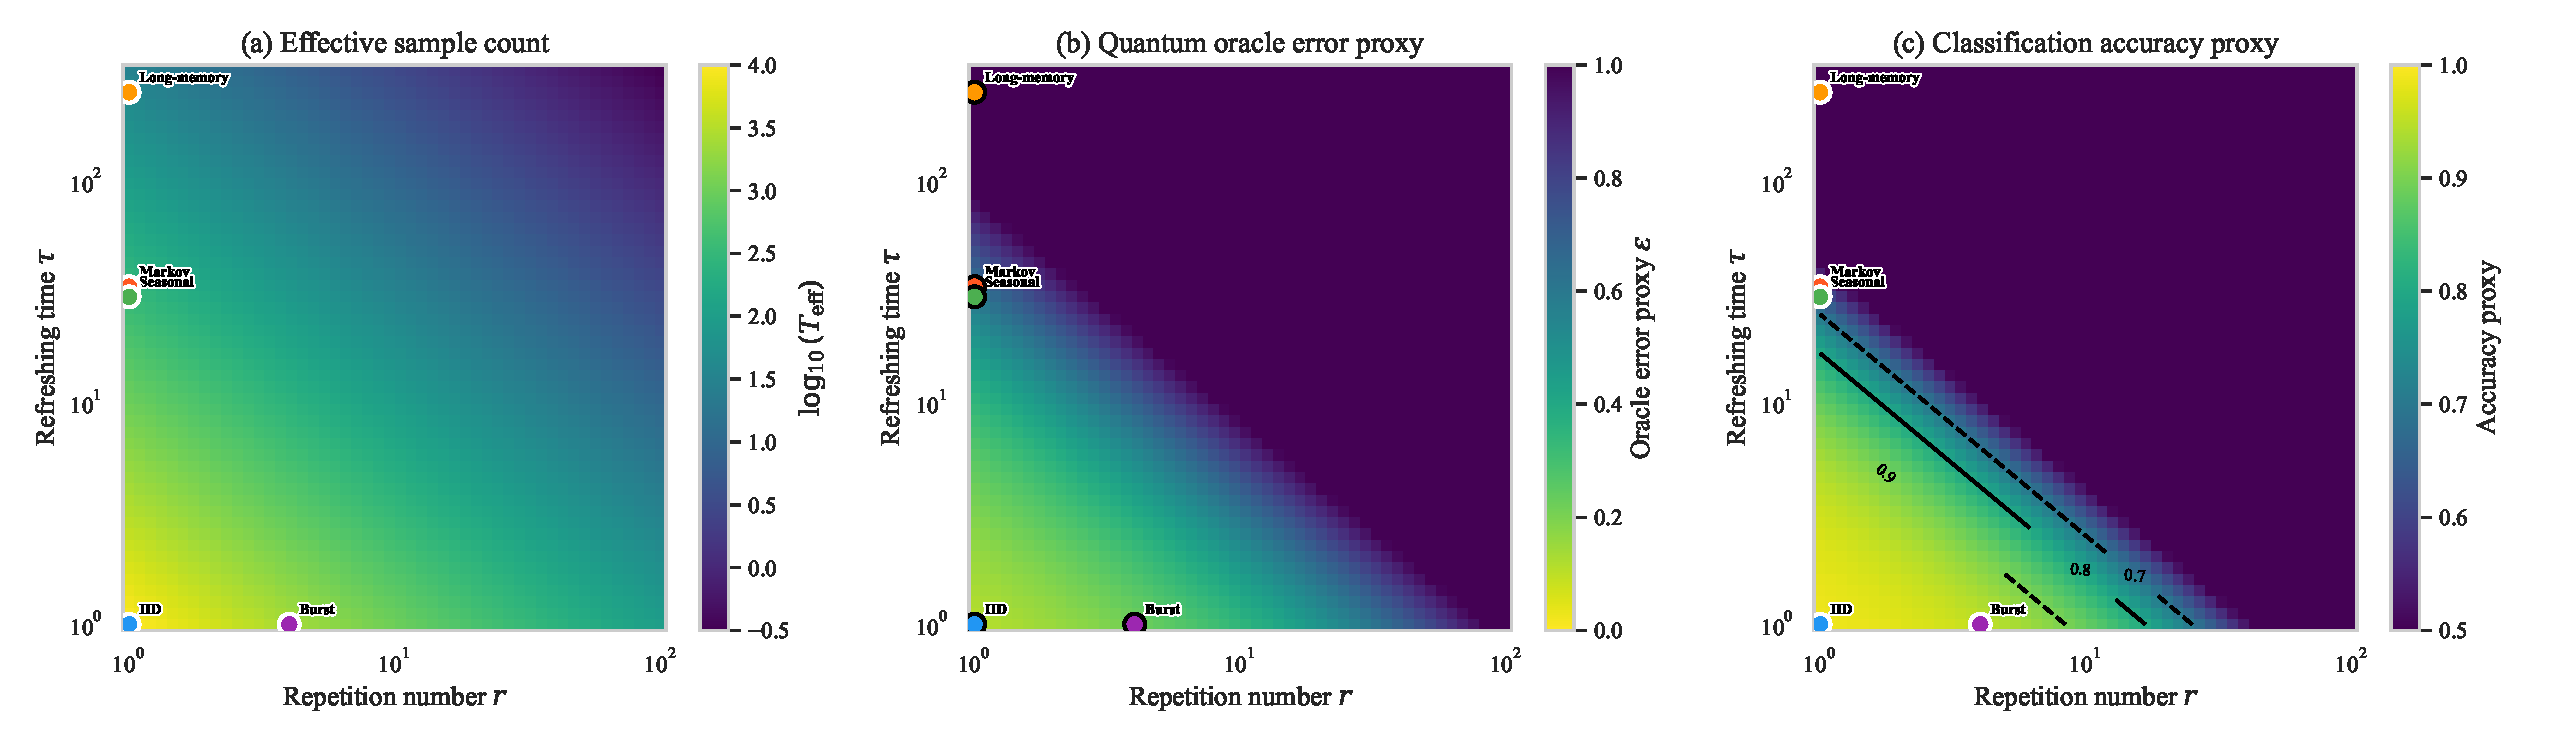
\includegraphics[width=\textwidth]{fig3_tau_r_landscape.pdf}
    \caption{Sensitivity landscape in $(\tau, r)$ space ($T = 10{,}000$, $n = 10$). \textbf{(a)} $\Teff = T/(\tau r)$, log$_{10}$ scale. \textbf{(b)} Oracle error proxy $\epsilon$. \textbf{(c)} Classification accuracy proxy with contours at $0.7$, $0.8$, $0.9$; colored dots mark each regime's analytic $(\tau, r)$.}
    \label{fig:landscape}
\end{figure}

$\Teff$ decreases diagonally as $\tau$ and $r$ increase; accuracy contours follow hyperbolas in $\tau \cdot r$ space. IID and burst fall in the high-accuracy corner; Markov and seasonal sit near the $0.7$--$0.8$ contour; long-memory falls in the low-accuracy zone. Researchers can place estimated $(\tau, r)$ values on the landscape to identify comparable synthetic regimes for follow-on empirical or algorithm-level validation.

\subsection{Experiment 4: Empirical vs.\ Proxy Correlation Parameters}
\label{sec:correlation_char}

\begin{figure}[t]
    \centering
    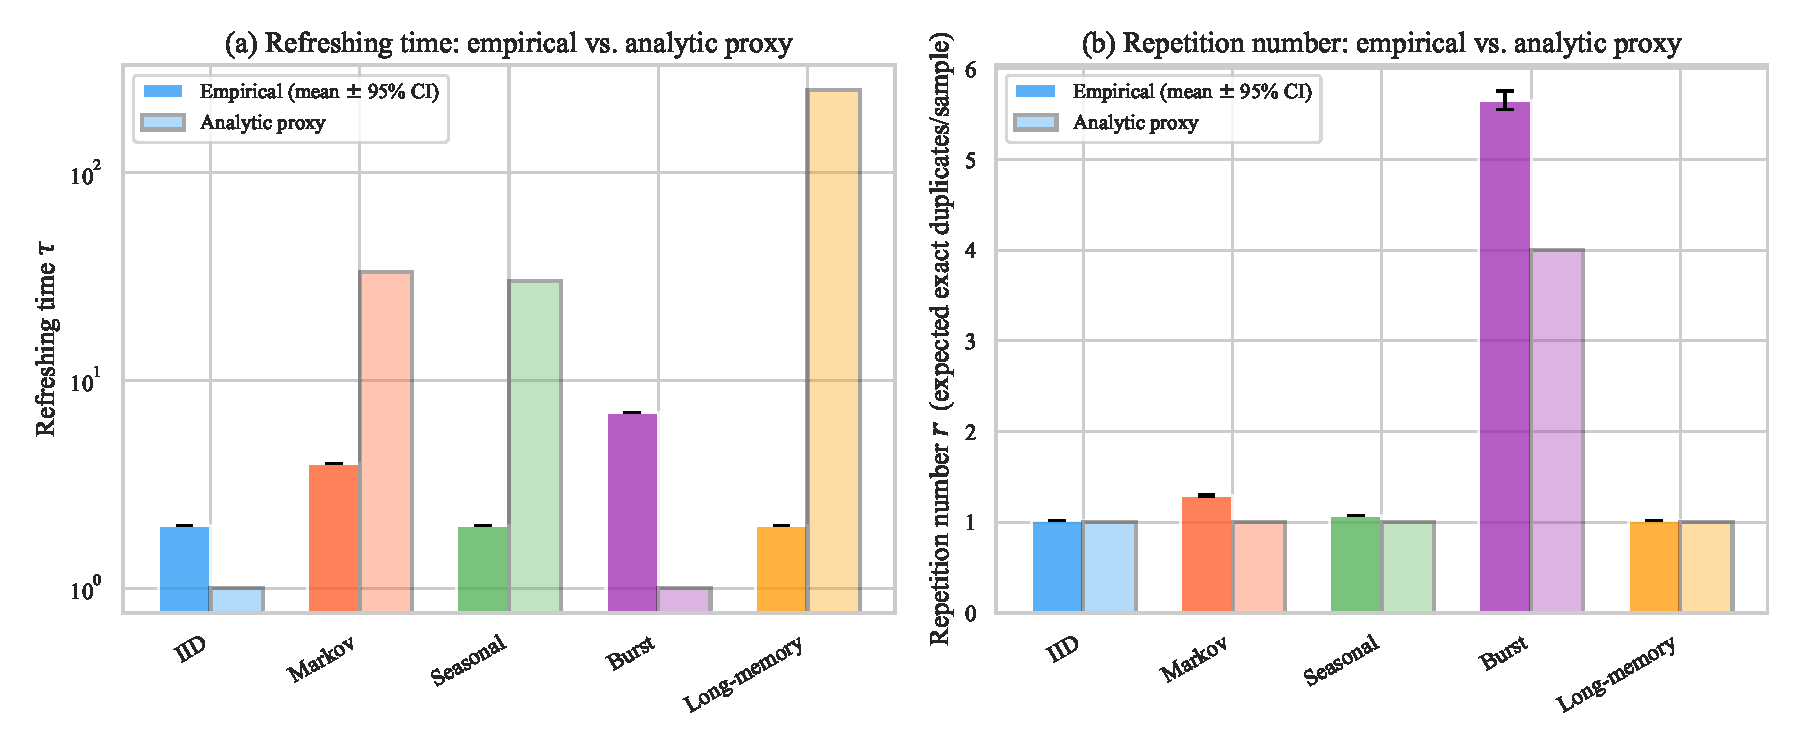
\includegraphics[width=0.85\textwidth]{fig4_correlation_characterization.pdf}
    \caption{Empirical vs.\ analytic proxy $\tau$ and $r$ (10-seed mean $\pm$ 95\% CI). \textbf{(a)} Refreshing time $\tau$: analytic exceeds empirical for Markov, seasonal, long-memory; opposite for IID and burst. \textbf{(b)} Repetition number $r$: both quantities in units of expected exact duplicate copies per sample within a $W=20$ forward window.}
    \label{fig:corr_char}
\end{figure}

Three findings emerge from Fig.~\ref{fig:corr_char}. First, analytic $\tau$ systematically overshoots empirical $\tau$: Markov ($33$ vs.\ $4$, $\approx 8\times$), long-memory ($251$ vs.\ $2$, $\approx 125\times$, explained by the arcsine relationship from binarisation \citep{beran1994statistics,mandelbrot1968fbm}), and seasonal ($30$ vs.\ $2$); IID and burst show the opposite sign from finite-sample fluctuations. Second, unit-aligned $r$ values agree well: burst empirical $r \approx 5.6$ vs.\ analytic $r = 4$ (factor $1.4\times$, attributable to window-length choice); all other regimes near 1. Third, IID ($\tau_{\text{emp}} \approx 2$ vs.\ $\tau_{\text{analytic}} = 1$) sets the finite-sample noise floor. These findings confirm that $(\tau, r)$ are qualitatively informative but quantitatively loose; family-specific refinements would enlarge the predicted favourable region.

\subsection{Experiment 5: Correlation Strength Sweep}
\label{sec:sweep}

Figure~\ref{fig:markov_sweep} examines how the classical-vs-proxy separation evolves as the Markov correlation strength $\rho$ is varied continuously from 0 (IID) to 0.95 (strong correlation), comparing the classical SGD baseline against the quantum proxy using both the \emph{analytic} $\tau$ and the \emph{empirically measured} $\tau$.

\begin{figure}[t]
    \centering
    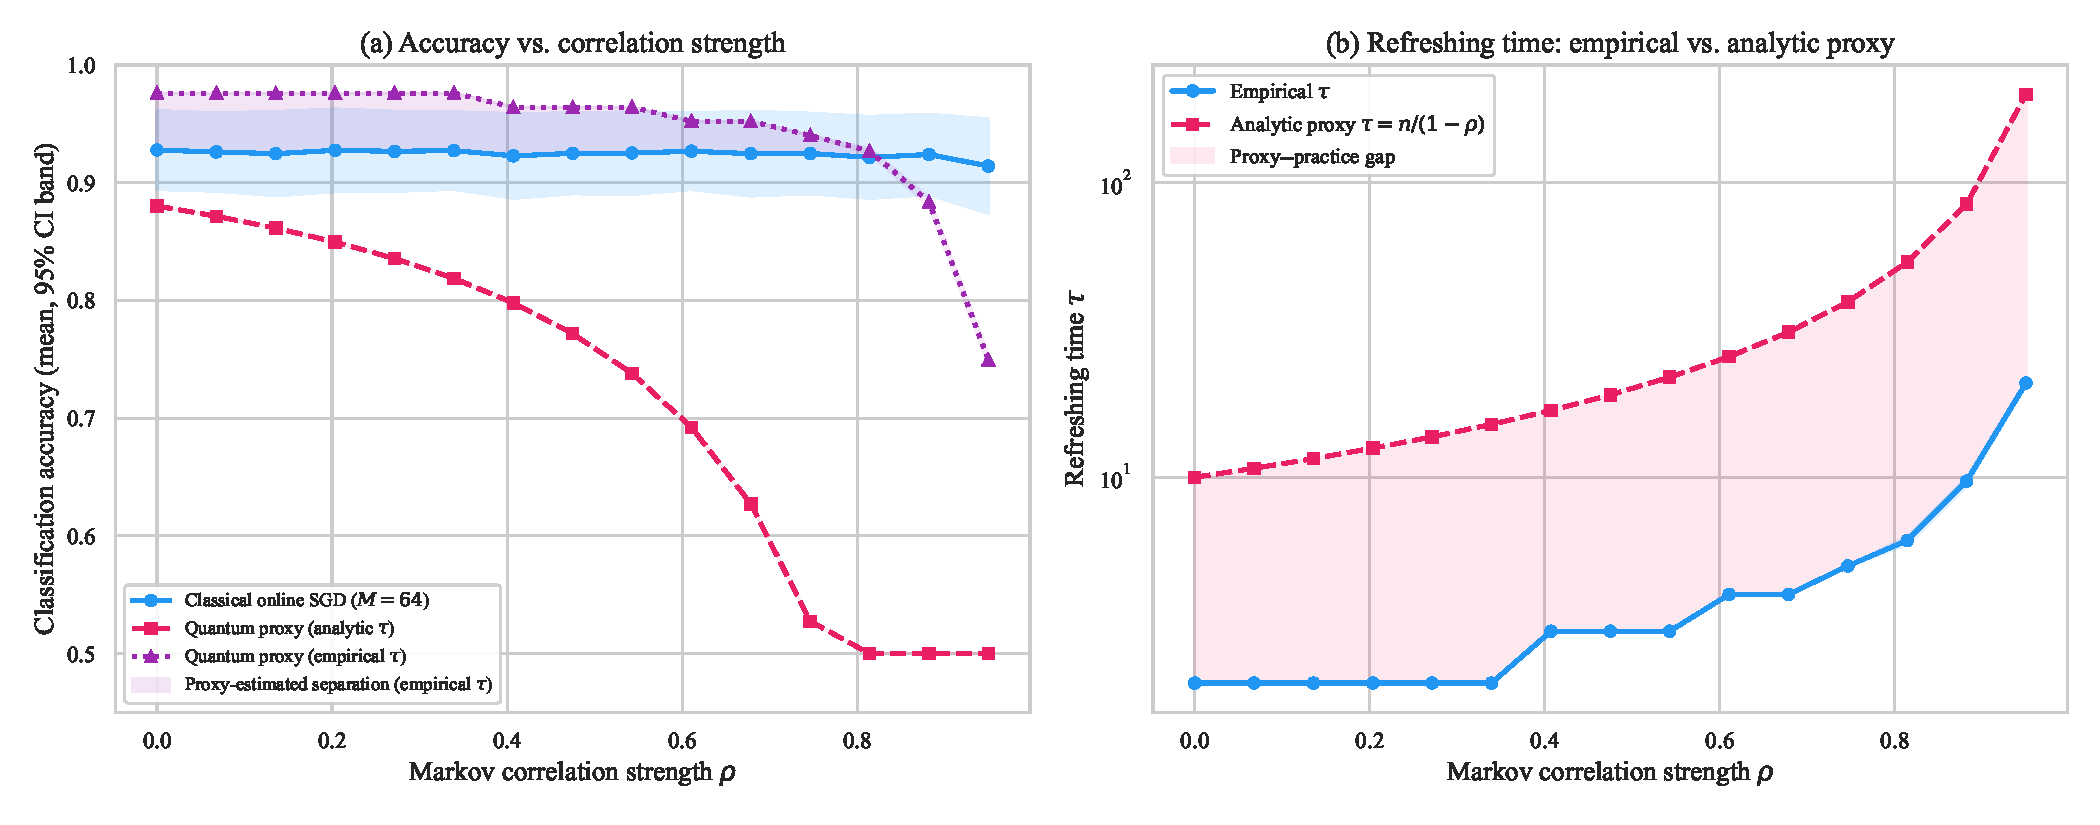
\includegraphics[width=\textwidth]{fig5_markov_sweep.pdf}
    \caption{Markov correlation strength sweep (10-seed mean with 95\% CI bands). \textbf{(a)} Classification accuracy: classical online SGD at $M = 64$ (blue) is approximately flat at ${\sim}0.92$ across the sweep. The quantum accuracy proxy using the \emph{analytic} $\tau = n/(1{-}\rho)$ (pink, dashed) degrades and crosses below classical at moderate $\rho$ near the lower end of the sweep. The quantum proxy using the \emph{empirical} $\tau$ (purple, dotted) remains above classical until $\rho \approx 0.88$, indicating that tighter family-specific characterisations would enlarge the region in which the proxy model predicts a favourable separation. \textbf{(b)} Refreshing time: the proxy--practice gap (shaded) grows with $\rho$, showing that the analytic proxy is increasingly conservative under stronger correlation. CI bands are narrow throughout, confirming that the main trends are seed-stable.}
    \label{fig:markov_sweep}
\end{figure}

Panel~(a) reveals a key insight: using the analytic proxy $\tau$, the quantum performance proxy crosses below classical performance at $\rho \approx 0.3$, suggesting the proxy-model crossover occurs under moderate Markov correlation. However, using empirical $\tau$ instead, the empirical-$\tau$ proxy remains above $0.9$ for $\rho \leq 0.8$ and above the classical baseline across most of the sweep. Under the empirical-proxy model, the classical baseline first becomes statistically indistinguishable from the proxy near $\rho \approx 0.68$ and significantly exceeds it by $\rho \approx 0.88$ (see Table~\ref{tab:markov_summary} for paired Wilcoxon $p$-values); the proxy-model crossover therefore occurs near $\rho \approx 0.88$, where even the empirical autocorrelation becomes severe.

Panel~(b) quantifies the source of this discrepancy: the analytic proxy $\tau = n/(1{-}\rho)$ grows as a pole at $\rho = 1$, while the empirical $\tau$ grows much more gradually. The shaded proxy--practice gap widens by over an order of magnitude at $\rho = 0.9$. This gap is the primary driver of the pessimistic quantum performance proxies observed in Experiments~1--3, and its characterization is one of the central contributions of this paper.

\begin{table}[t]
\centering
\caption{Classical-vs-proxy comparison across representative Markov correlation strengths $\rho$: empirical classical online-SGD accuracy at $M = 64$, the heuristic quantum accuracy proxy using the empirically measured $\tau$, 10-seed half-width of the 95\% CI, and the paired Wilcoxon signed-rank $p$-value (two-sided). ``Proxy $>$ classical'' means the proxy estimate exceeds the empirical classical baseline, not realized quantum algorithmic superiority. Significant differences are marked with $^{\star}$ ($p < 0.05$). Accuracies are reported as mean $\pm$ half-width.}
\label{tab:markov_summary}
\begin{tabular}{lccccc}
\hline
$\rho$ & Classical SGD & Quantum proxy (emp.\ $\tau$) & $\Delta$ & Wilcoxon $p$ & Significance \\
\hline
$0.00$ & $0.928 \pm 0.034$ & $0.976 \pm 0.000$ & $+0.048$ & $0.020$ & $^{\star}$ proxy $>$ classical \\
$0.27$ & $0.927 \pm 0.034$ & $0.976 \pm 0.000$ & $+0.049$ & $0.027$ & $^{\star}$ proxy $>$ classical \\
$0.47$ & $0.925 \pm 0.034$ & $0.964 \pm 0.000$ & $+0.039$ & $0.049$ & $^{\star}$ proxy $>$ classical \\
$0.68$ & $0.925 \pm 0.036$ & $0.952 \pm 0.000$ & $+0.027$ & $0.375$ & not significant \\
$0.88$ & $0.924 \pm 0.034$ & $0.884 \pm 0.004$ & $-0.040$ & $0.037$ & $^{\star}$ classical $>$ proxy \\
\hline
\end{tabular}
\end{table}

\paragraph{Stability of the proxy-baseline crossover} These tests compare an empirical classical learner against a deterministic proxy pipeline, not two empirical algorithms; they establish the stability of the proxy-baseline crossover, not quantum superiority. For each correlation strength $\rho$ in the sweep, the paired observations are the per-seed empirical classical accuracy (10 seeds) and the deterministic proxy value at that $\rho$ (which is identical across seeds because the proxy is a closed-form function of empirically measured $\tau$ and $r$, not of any classical model state). The Wilcoxon $p$-value therefore tests whether the seed-to-seed variability of the empirical learner is consistent with a fixed offset relative to the proxy curve, not whether one implemented algorithm beats another. Paired Wilcoxon tests confirm that the crossover is not a seed artefact: the proxy significantly exceeds classical at $\rho \in \{0, 0.27, 0.47\}$ ($p \leq 0.049$), the two curves are indistinguishable at $\rho = 0.68$ ($p = 0.375$), and classical significantly exceeds the proxy at $\rho = 0.88$ ($p = 0.037$; Table~\ref{tab:markov_summary}).

\subsection{Experiment 6: Dimension Scaling}

Figure~\ref{fig:scaling} illustrates the exponential scaling of the quantum-vs-classical memory gap with data dimension.

\begin{figure}[t]
    \centering
    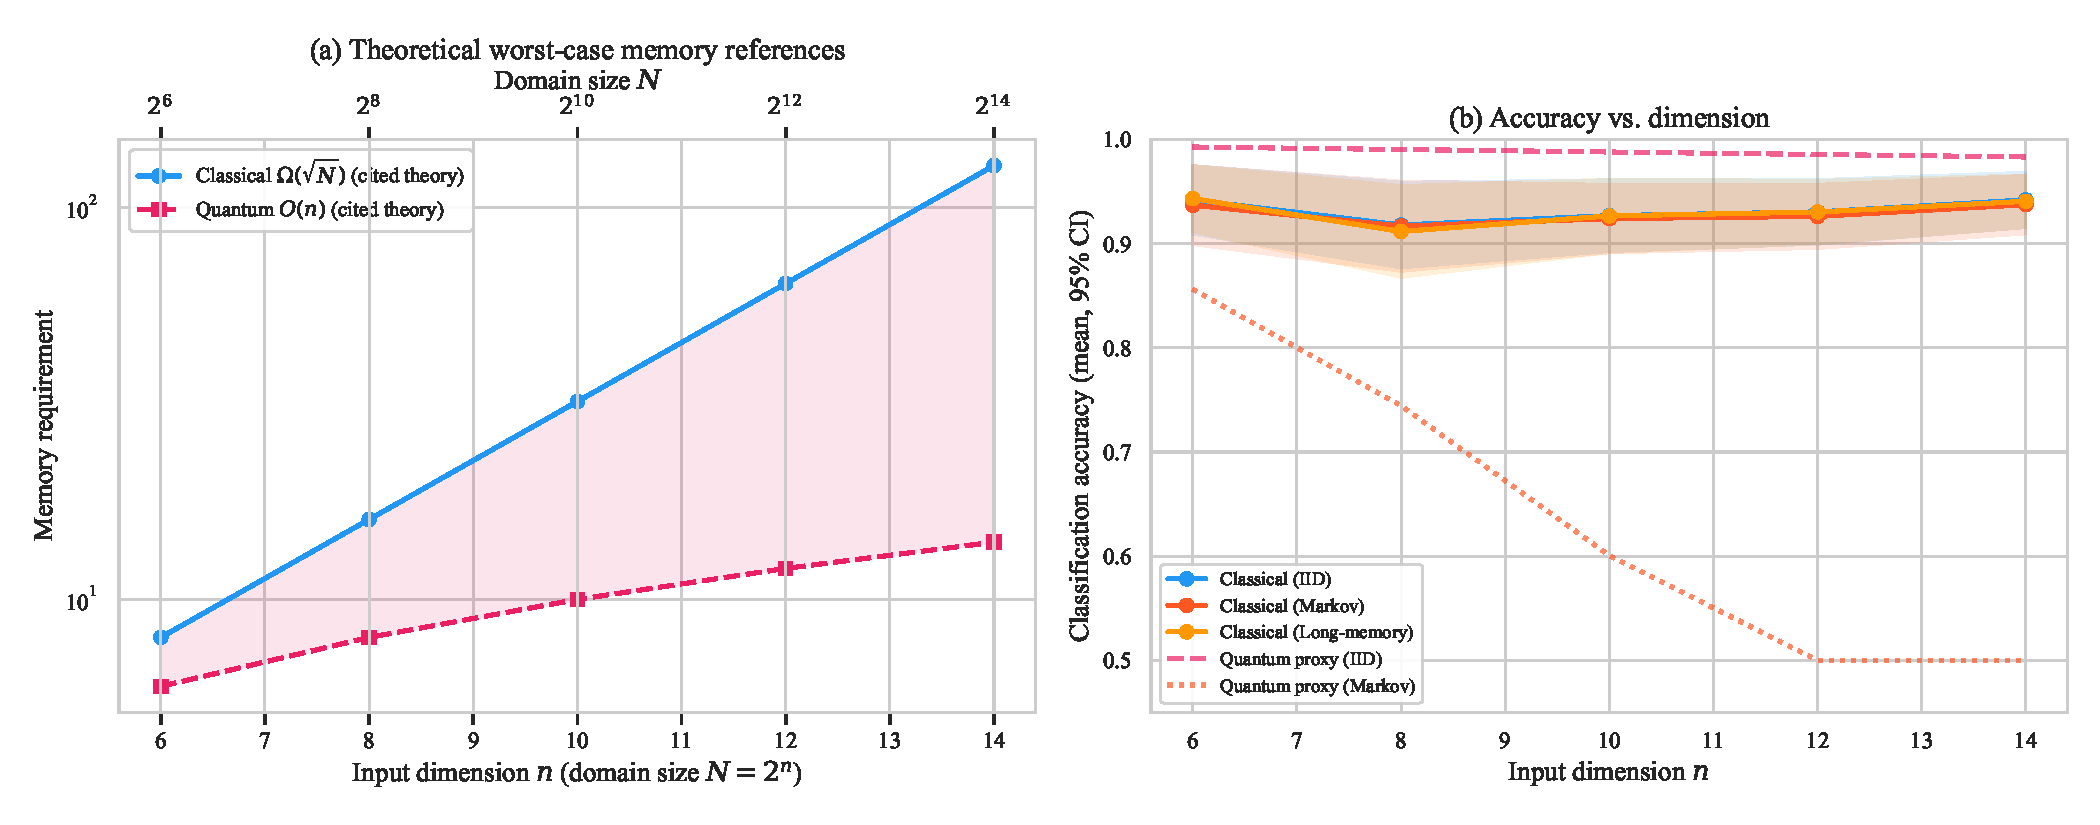
\includegraphics[width=\textwidth]{fig6_dimension_scaling.pdf}
    \caption{Dimension scaling analysis (10-seed mean, 95\% CI bands). \textbf{(a)} Worst-case memory reference: representative classical lower bound $\Omega(\sqrt{N}) = \Omega(2^{n/2})$ vs.\ quantum $\bigO(n)$. The gap is exponential in $n$; this is a worst-case reference, not a witnessed empirical floor. \textbf{(b)} Classification accuracy vs.\ dimension $n$: classical online-SGD accuracy for IID, Markov, and long-memory data (solid lines) compared with quantum accuracy proxies for IID and Markov (dashed). The quantum IID proxy is consistently near $1.0$; the quantum Markov proxy degrades with dimension (because $\tau_{\text{Markov}} = n/(1{-}\rho)$ grows with $n$, reducing $\Teff$), while classical accuracy is approximately stable across the range studied.}
    \label{fig:scaling}
\end{figure}

Panel~(a) shows that at $n = 14$ ($N = 16{,}384$) the representative classical memory reference exceeds 128 while the quantum requirement is only 14 qubits --- an exponential gap that widens with $n$ (the $\Omega(\sqrt{N})$ floor is a worst-case reference, not an empirical floor; see Section~\ref{sec:heuristic_model}). Panel~(b) shows that classical SGD accuracy is approximately stable across $n \in [6, 14]$, while the quantum IID proxy is consistently near $1.0$. The quantum Markov proxy \emph{decreases} with dimension because $\tau_{\text{Markov}} = n/(1-\rho)$ grows linearly with $n$; family-specific proxy refinements are therefore most useful at higher dimensions.

\subsection{Experiment 7: Rolling Accuracy Dynamics}

\begin{figure}[t]
    \centering
    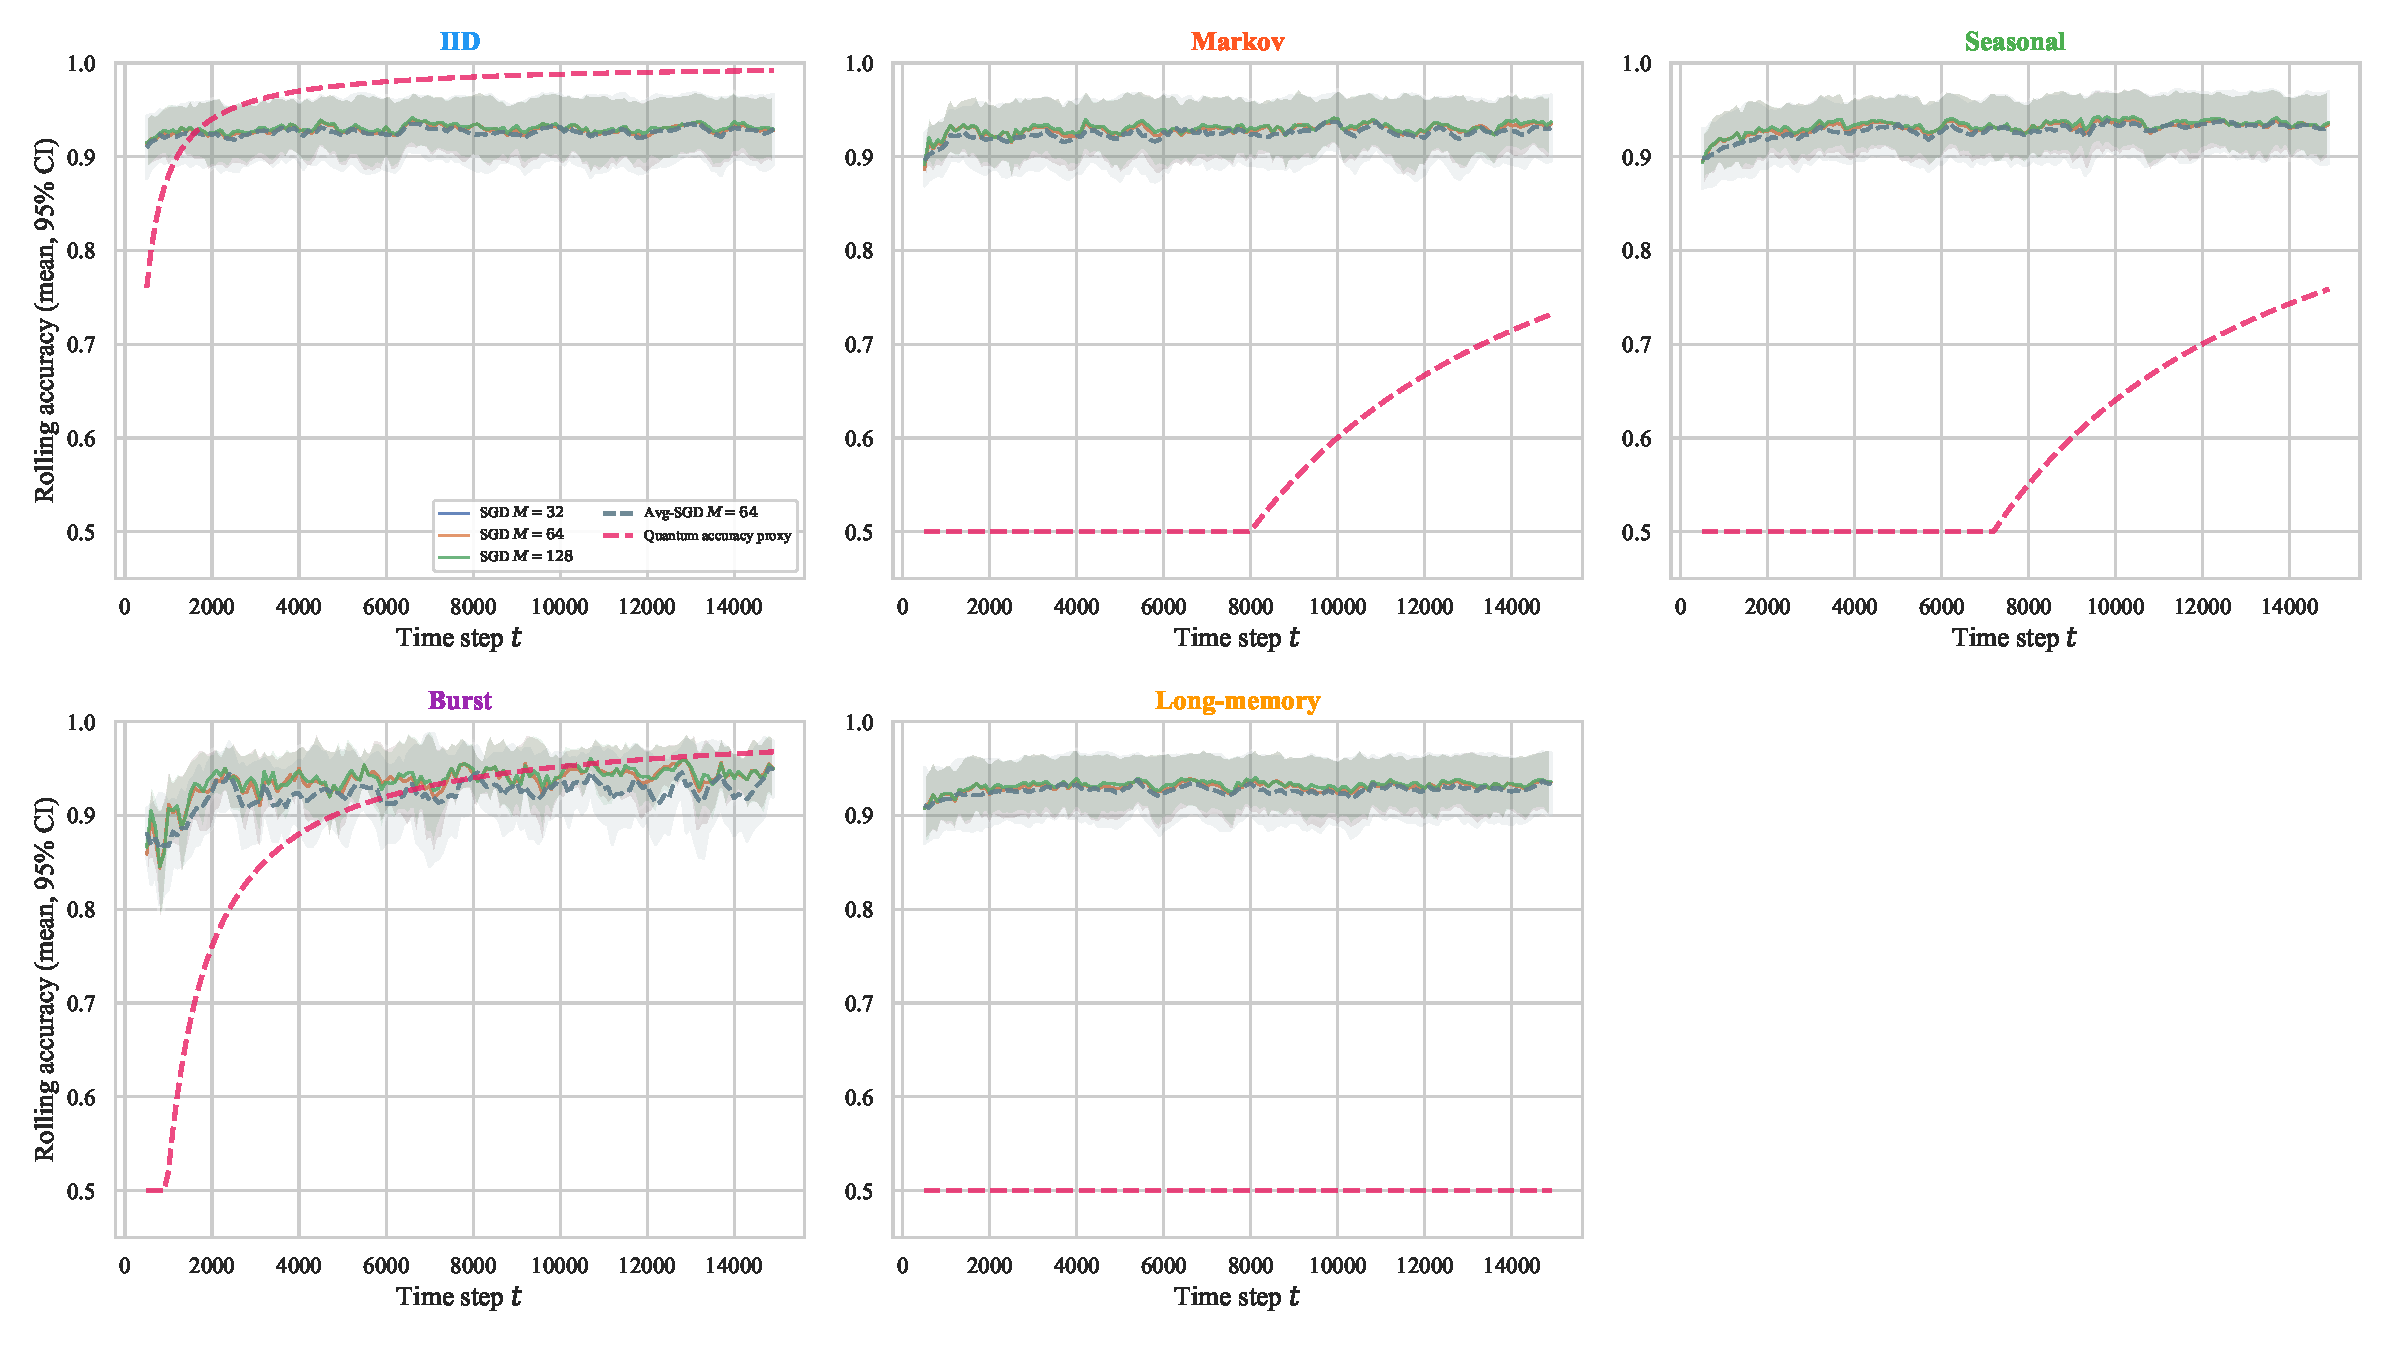
\includegraphics[width=\textwidth]{fig7_rolling_accuracy.pdf}
    \caption{Rolling accuracy (window $= 500$) per regime; 10-seed mean $\pm$ 95\% CI. Classical SGD at $M \in \{32, 64, 128\}$ (solid), averaged SGD $M = 64$ (dashed grey), quantum proxy (dashed pink). Under IID and burst the proxy reaches or exceeds classical by horizon end; under Markov and seasonal it rises more slowly and remains below classical (conservative analytic $\tau$); under long-memory the proxy is pinned at $0.5$ throughout.}
    \label{fig:rolling}
\end{figure}

Figure~\ref{fig:rolling} confirms the regime-dependent pattern of Experiments~1 and 5: IID and burst show higher proxy-estimated trajectories; Markov and seasonal show a visible gap attributable to the conservative analytic $\tau$ (a tighter family-specific proxy would shift the trajectory upward, as the Markov sweep confirms); long-memory exhibits the $0.5$ saturation floor and persistent low-frequency classical oscillations characteristic of long-range dependence.


\subsection{Experiment 8: Real-Stream Sanity Check}
\label{sec:real_stream}

The synthetic experiments above leave open whether the empirical $\tau$ and $r$ estimators apply usefully to real streams. To answer this we apply the proxy framework end-to-end to two publicly available real streams from the Numenta Anomaly Benchmark \citep{ahmad2017numenta} (NAB; MIT licence) and report what is observed. No claim of quantum advantage is made; the contribution of this experiment is the successful application of the diagnostic workflow outside the synthetic regime, not a comparison against a realised quantum algorithm. The two streams were chosen \emph{before} examining the results to span very different correlation regimes (transport-traffic seasonality versus industrial-sensor drift), and we pre-committed to reporting whichever placement and baseline outcomes emerged.

\paragraph{Datasets} (i) \emph{NYC Taxi}: $T = 10{,}320$ half-hour pickup counts in New York City (2014-07-01 to 2015-01-31). Combines strong daily/weekly seasonality with documented burst events (NYC Marathon, Thanksgiving, snowstorms); overlaps the synthetic seasonal $+$ burst $+$ low-order Markov regimes. (ii) \emph{Machine Temperature}: $T = 22{,}695$ five-minute readings from an industrial machine sensor preceding a documented system failure. Exhibits slow drift over hours-to-days plus localised spike events; overlaps the long-memory $+$ burst regimes.

\paragraph{Binarisation choice} Each continuous series is encoded into $n = 6$ binary features (matched to Section~\ref{sec:ablations}): a 3-bit time-of-day bucket, a weekend flag, and two trend bits (current and lag-1 indicator of whether the value exceeds a 7-day rolling median; the rolling window is $336$ bins for NYC Taxi at 30-min resolution and $2{,}016$ bins for Machine Temperature at 5-min resolution). The target $y_t$ is a simple rare-event classification proxy: $y_t = 1$ iff the next-bin value is at or above the 80th percentile of the full series. \emph{This is a per-stream high-activity threshold and not the original NAB anomaly label.} The 80th percentile is chosen because it produces a non-trivial $\sim$20\%/80\% class imbalance that exposes both majority-baseline behaviour and the rare-event regime; this target is intentionally imbalanced and not a balanced classification task. To prevent accuracy from masking majority-class memorisation, we report balanced accuracy and $F_1$ of the positive (rare) class alongside accuracy in Table~\ref{tab:real_stream_metrics}. Sensitivity to this threshold ($q \in \{0.70, 0.80, 0.90\}$) is recorded in the JSON output for transparency. Binarisation discards information, so the resulting empirical $\tau$ and $r$ should be read as lower bounds on the correlation lengths in the underlying continuous process.

\paragraph{Procedure} Empirical $\tau$ and $r$ are computed using the same estimators as the synthetic experiments (Section~\ref{sec:experiments}). The three classical baselines are run with $M = 64$ on seed-permuted prequential orders (10 seeds, 95\% confidence intervals). The proxy accuracy is $\mathrm{acc\_proxy} = \max(0.5, 1 - C^2 n \log(1/\delta) / \Teff)$ with $C = 2$, $\delta = 0.05$.

\paragraph{Findings (Tables~\ref{tab:real_stream} and \ref{tab:real_stream_metrics})} The two streams land on opposite sides of the proxy-favourable region in $(\tau, r)$ space, and the imbalance-aware metrics expose effects that accuracy alone hides:
\begin{itemize}
    \item \textbf{NYC Taxi} (favourable region): $\tau_{\text{emp}} = 6.0$, $r_{\text{emp}} = 2.77$, $\Teff = 621$, proxy $= 0.884$. Count-Min reaches accuracy $0.865 \pm 0.016$, balanced accuracy $0.777$, and $F_1 = 0.644$, materially above majority on every metric. Online-SGD and Averaged-SGD have lower accuracy ($0.670 \pm 0.006$ and $0.673 \pm 0.004$) and balanced accuracy near $0.50$, indicating they recover the rare class only weakly under hashed-linear features.
    \item \textbf{Machine Temperature} (unfavourable region): $\tau_{\text{emp}} = 32.0$, $r_{\text{emp}} = 13.55$, $\Teff = 52$, proxy $= 0.500$ (saturated at the chance floor). All three classical baselines have accuracy near the majority value ($0.724$, $0.735$, $0.801$), but balanced accuracy is only $0.55$, $0.54$, and $0.56$ and $F_1 \in [0.23, 0.27]$. The accuracy gap above the saturated proxy is therefore largely majority-class memorisation; on the imbalance-aware metrics no classical baseline meaningfully exceeds chance for the rare class.
\end{itemize}

\begin{table}[t]
\centering
\caption{Real-stream sanity check, landscape coordinates: empirical $(\tau, r)$, proxy accuracy, classical-baseline accuracy (10-seed mean), and the majority-class accuracy for two NAB datasets. The proxy places NYC Taxi in a favourable region and Machine Temperature in an unfavourable region (proxy saturates at $0.5$). Imbalance-aware metrics (balanced accuracy, $F_1$) for the same runs are reported separately in Table~\ref{tab:real_stream_metrics}.}
\label{tab:real_stream}
\begin{tabular}{@{}lrrrrcccc@{}}
\toprule
Dataset & $T$ & $\tau$ & $r$ & $\Teff$ & proxy & SGD & Avg-SGD & Count-Min \\
\midrule
NYC Taxi          & $10{,}320$ & $6.0$  & $2.77$  & $621$ & $0.884$ & $0.670$ & $0.673$ & $0.865$ \\
Machine Temp.\    & $22{,}695$ & $32.0$ & $13.55$ & $52$  & $0.500$ & $0.724$ & $0.735$ & $0.801$ \\
\bottomrule
\end{tabular}
\end{table}

\begin{table}[t]
\centering
\caption{Imbalance-aware metrics for the real-stream sanity check (10-seed mean). Accuracy alone is misleading at a $\sim$20\%/80\% positive/negative split, so balanced accuracy and $F_1$ of the positive (rare) class are reported alongside it. The proxy is an accuracy projection only; balanced accuracy and $F_1$ are reported for the classical baselines and are not targets the proxy attempts to match. On NYC Taxi, Count-Min materially exceeds majority on every metric. On Machine Temperature, all classical baselines have accuracy slightly above majority but balanced accuracy near $0.5$ and $F_1 < 0.30$, indicating the accuracy gap is largely majority-class memorisation.}
\label{tab:real_stream_metrics}
\begin{tabular}{@{}llccc@{}}
\toprule
Dataset & Method & accuracy & balanced acc.\ & $F_1$ (positive) \\
\midrule
NYC Taxi              & majority           & $0.800$ & $0.500$ & $0.000$ \\
                      & Online-SGD         & $0.670$ & $0.535$ & $0.273$ \\
                      & Averaged-SGD       & $0.673$ & $0.498$ & $0.199$ \\
                      & Count-Min          & $0.865$ & $0.777$ & $0.644$ \\
\midrule
Machine Temperature   & majority           & $0.800$ & $0.500$ & $0.000$ \\
                      & Online-SGD         & $0.724$ & $0.550$ & $0.269$ \\
                      & Averaged-SGD       & $0.735$ & $0.538$ & $0.234$ \\
                      & Count-Min          & $0.801$ & $0.560$ & $0.228$ \\
\bottomrule
\end{tabular}
\end{table}

\begin{figure}[t]
    \centering
    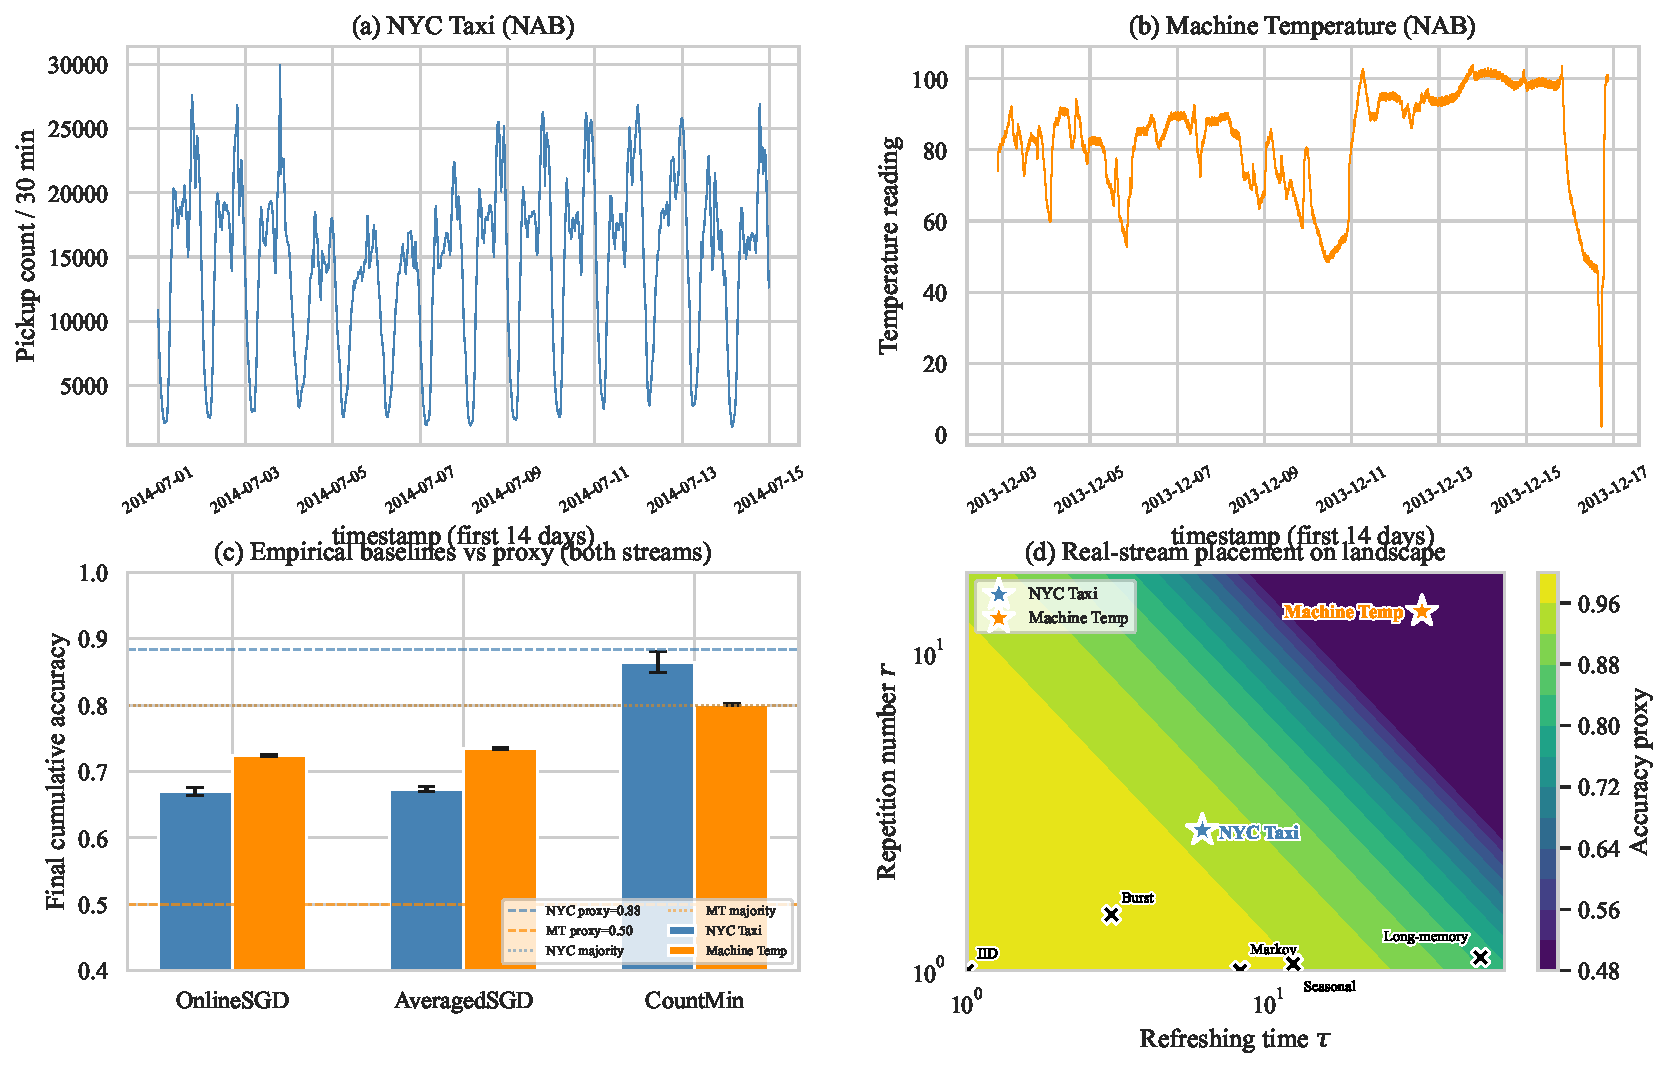
\includegraphics[width=\textwidth]{fig8_real_stream_validation.pdf}
    \caption{Real-stream sanity check (two NAB datasets). \textbf{(a, b)} Raw series for the first 14 days of each dataset. \textbf{(c)} Final cumulative classical baseline accuracy (10-seed mean $\pm$ 95\% CI) for both streams; dashed lines are the deterministic proxy values, dotted lines are the majority baseline. \textbf{(d)} Both real-stream points (coloured stars) on the $(\tau, r)$ landscape, alongside synthetic-regime markers (white crosses). NYC Taxi falls in a moderately favourable region near the synthetic Markov point; Machine Temperature falls in the unfavourable upper-right region (high $\tau$ and very high $r$) where the proxy saturates. Imbalance-aware metrics for the same runs are reported in Table~\ref{tab:real_stream_metrics}.}
    \label{fig:real_stream}
\end{figure}

\paragraph{Why Count-Min looks strong on NYC Taxi} The near-proxy accuracy of Count-Min on NYC Taxi has a structural explanation that is worth stating up front, because otherwise the apparent agreement could be misread as evidence that the proxy is ``correct''. With $n = 6$ binary features only $2^n = 64$ feature vectors exist, and many of them repeat in the data; Count-Min can therefore essentially memorise per-bucket positive rates and predict the majority class for each bucket, which is enough to reach $F_1 = 0.644$ at this binarisation granularity. SGD with hashed-linear features cannot represent the same per-bucket conditional distribution as efficiently. The Count-Min result should be interpreted as a memorisation-friendly bounded-memory baseline under coarse binarisation, not as general evidence that the proxy predicts all classical learners. As $n$ grows, $2^n$ outpaces practical Count-Min table sizes and this memorisation route disappears.

\paragraph{Interpretation} Three observations.
(i) The empirical $\tau$ and $r$ estimators apply unchanged to both real streams and place each stream in the regime that matches its underlying structure: NYC Taxi has moderate $\tau$ (multiple-bin daily/weekly correlation) and moderate $r$ (modest exact-feature-vector repetition at $n = 6$); Machine Temperature has high $\tau$ (slow multi-hour drift) and very high $r$ (5-min sensor data has many near-identical consecutive feature vectors).
(ii) On NYC Taxi, Count-Min materially exceeds the majority baseline on balanced accuracy ($0.777$ vs.\ $0.500$) and on $F_1$ ($0.644$ vs.\ $0.000$), so the accuracy match between Count-Min and the proxy reflects genuine rare-class learning rather than majority memorisation alone, even though the underlying mechanism is the bounded-$n$ memorisation route described above.
(iii) On Machine Temperature, the saturated proxy is exceeded by all classical baselines on accuracy, but the imbalance-aware metrics show that the gap is mostly majority-class memorisation: balanced accuracy is at most $0.56$ and $F_1$ is below $0.30$ for every classical baseline. This is the expected diagnostic behaviour at $\Teff = 52$---no sample-limited estimator should be expected to recover the rare class at this effective sample count---and we treat it as a genuine negative case.

The two streams together illustrate the value of the $(\tau, r)$ diagnostic: it identifies real streams that fall on either side of the proxy-favourable boundary using the same estimators applied to the synthetic regimes, and the imbalance-aware metrics confirm that the diagnostic is not an artefact of accuracy on imbalanced labels. Broader real-stream coverage across financial, network-traffic, and additional sensor domains remains future work (Section~\ref{sec:future_work}).


\subsection{Experiment 9: Proxy-Sensitivity and Estimator Ablations}
\label{sec:ablations}

To address the concern that several proxy choices appear ad hoc, we vary four ingredients of the pipeline and report whether the qualitative ordering of regimes on the $(\tau, r)$ landscape is preserved. All ablations use $T = 4096$, $W = 20$, and a feature dimension $n = 6$ chosen to match the real-stream case study (Section~\ref{sec:real_stream}) for direct comparability; the synthetic main experiments use $n = 10$, so absolute proxy values in this section are not directly comparable to those in Sections~\ref{sec:results}--\ref{sec:correlation_char}, but the qualitative regime ordering is.

\paragraph{Alternative $\tau$ estimators} Four definitions are compared: the default ($1/e$ ACF crossing), an aggressive variant ($1/2$ ACF crossing), the integrated absolute ACF up to first non-positive lag, and an AR(1) effective lag $-1/\log|\rho_1|$. The qualitative ordering is preserved across all five regimes: Burst always has the largest $\tau$ ($3.3$--$7.0$), IID and long-memory always the smallest ($1.0$--$2.0$), Markov consistently moderate ($2.8$--$4.0$). Resulting proxy accuracies (Table~\ref{tab:ablations}) shift by at most $0.04$ between estimators; the largest shift is in the Burst regime, where the proxy is in saturation and the AR(1) estimator yields a modestly higher value because it captures only the lag-1 dependence.

\paragraph{Forward-window size $W$} Repeating the $r$ estimator at $W \in \{10, 20, 50\}$ yields a monotone increase in $r$ (more chances to find duplicates) and a corresponding monotone decrease in $\Teff$. The relative ordering of regimes by $r$ is preserved across $W$ values, confirming that $W = 20$ is a representative choice.

\paragraph{Stream length $T$} Varying $T \in \{1024, 2048, 4096, 8192\}$ yields the expected scaling in $\Teff$. For Burst the proxy emerges from saturation only at $T \geq 8192$, indicating sample-size sensitivity for highly repetitive regimes.

\paragraph{Target function} On the linear target the SGD baseline degrades to near-chance ($\approx 0.5$) for these synthetic streams and the small $n=6$ feature set; on a threshold target ($y = 1$ iff $\sum_i x_i \geq n/2$) SGD attains $\approx 0.65$ across all regimes; on the parity target SGD remains near chance. The proxy model is target-independent (it depends only on $\Teff$), so this ablation isolates the gap between the proxy framework and the empirical learner's task-specific capability.

\begin{table}[t]
\centering
\caption{Proxy-sensitivity ablation: alternative $\tau$ estimators on synthetic streams ($T = 4096$, $W = 20$, $n = 6$). Qualitative ordering of regimes by $\tau$ is preserved across all four estimators; proxy accuracy changes by at most $0.04$.}
\label{tab:ablations}
\begin{tabular}{@{}lcccc@{}}
\toprule
Regime & $1/e$ (default) & $1/2$-cross & integrated & AR(1) eff. \\
\midrule
IID         & $0.954$ & $0.954$ & $0.977$ & $0.977$ \\
Markov $0.7$ & $0.856$ & $0.892$ & $0.877$ & $0.899$ \\
Seasonal    & $0.942$ & $0.942$ & $0.893$ & $0.971$ \\
Burst       & $0.500$ & $0.500$ & $0.500$ & $0.655$ \\
Long-memory & $0.954$ & $0.954$ & $0.977$ & $0.977$ \\
\bottomrule
\end{tabular}
\end{table}

\begin{figure}[t]
    \centering
    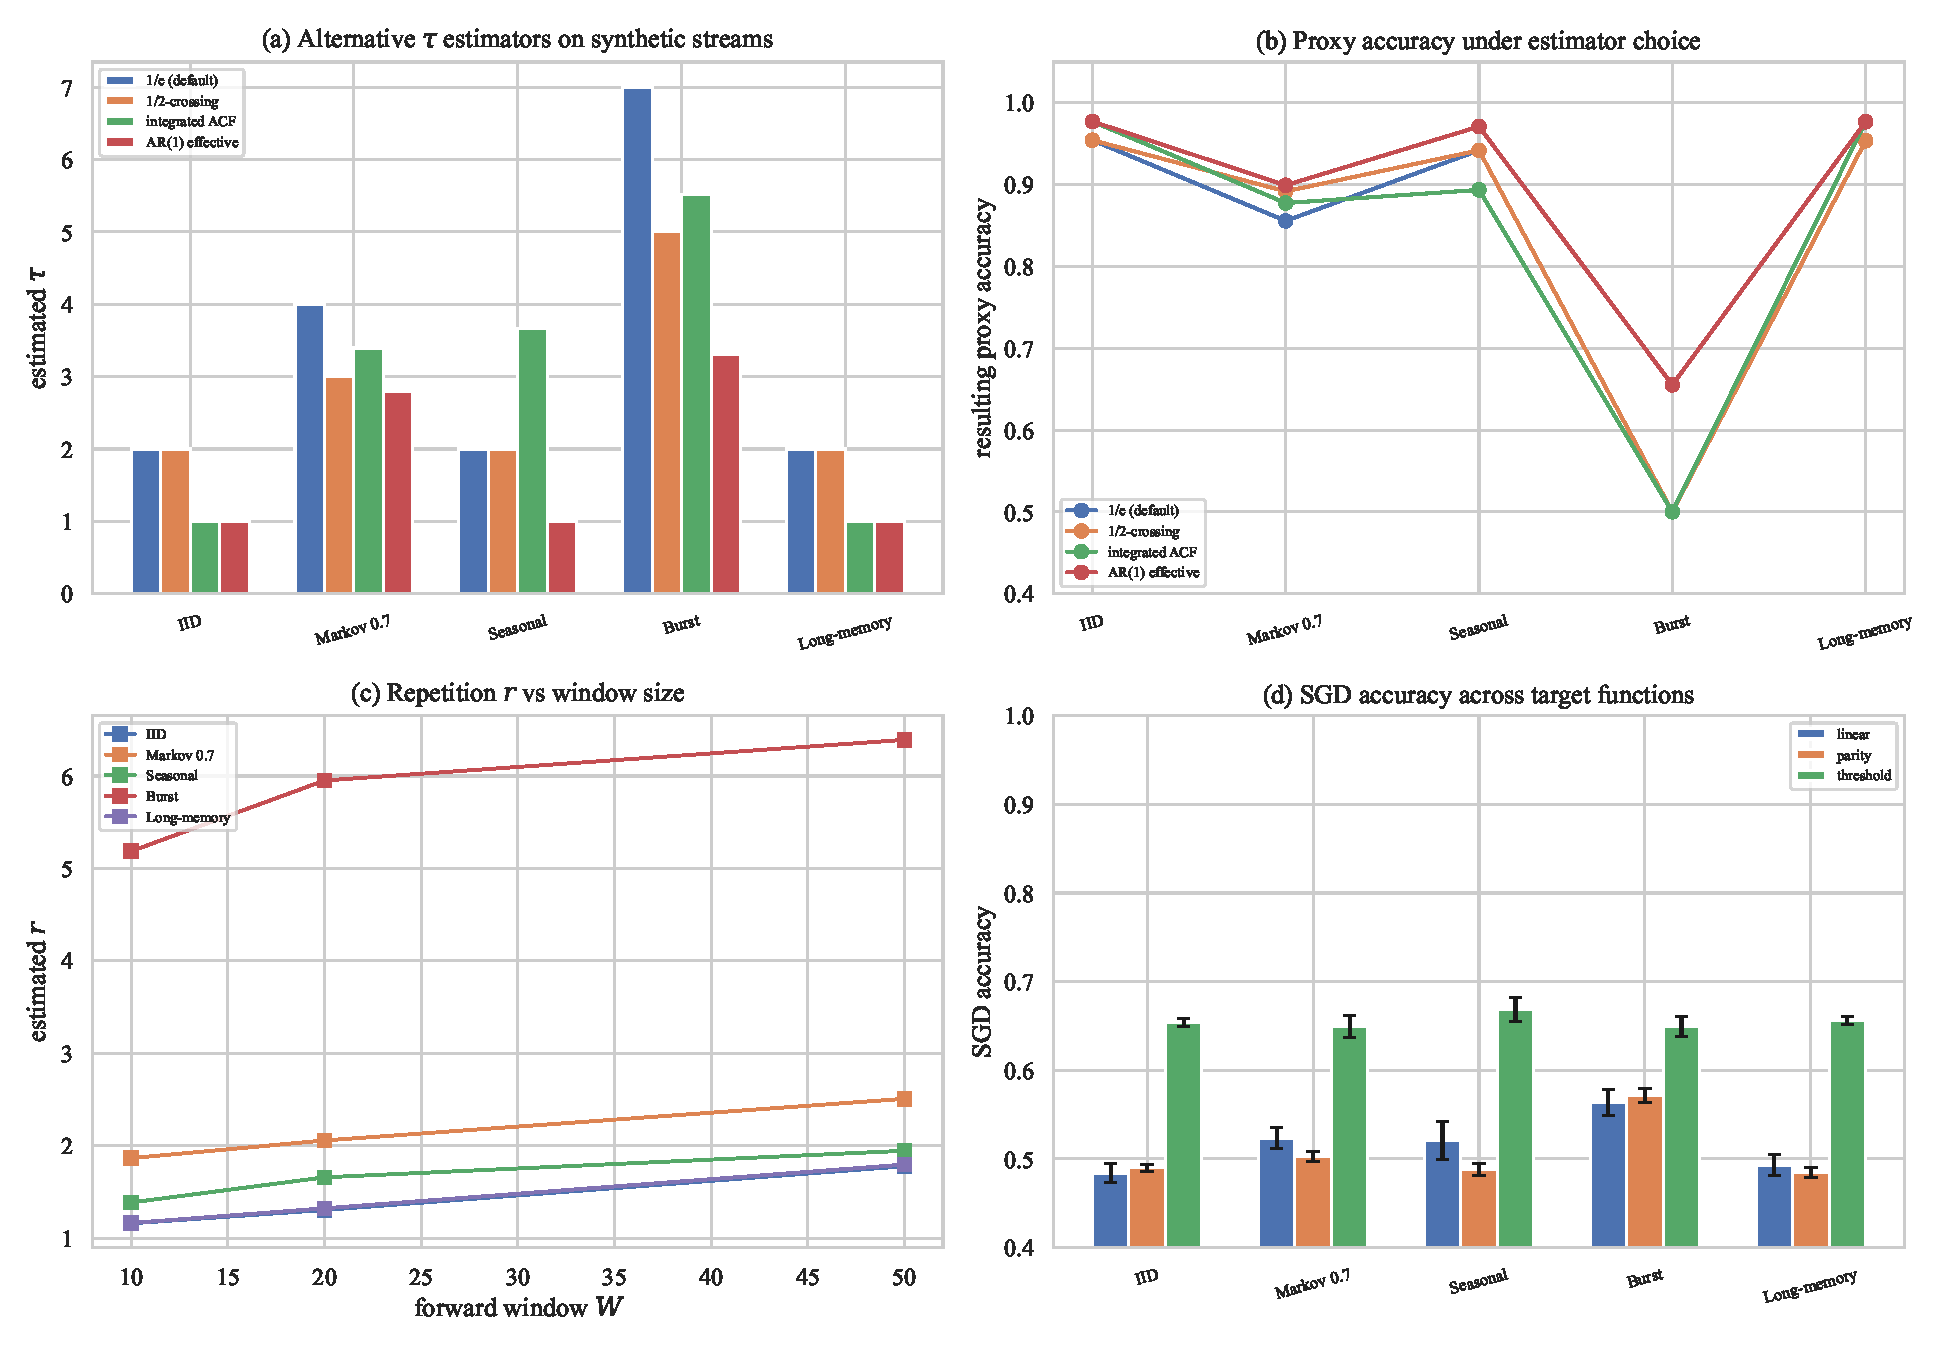
\includegraphics[width=\textwidth]{fig9_ablations.pdf}
    \caption{Proxy-sensitivity and estimator ablations. \textbf{(a)} Estimated $\tau$ on each regime under four alternative estimators (log scale). \textbf{(b)} Resulting proxy accuracy. \textbf{(c)} Repetition number $r$ versus forward-window size $W$. \textbf{(d)} Online-SGD accuracy across three target functions (linear, parity, threshold), 10-seed mean with 95\% CI. The proxy curve is target-independent.}
    \label{fig:ablations}
\end{figure}

Together these ablations show that the proxy model's qualitative regime ordering is robust to $\tau$ estimator choice and forward-window size, while the absolute proxy values are sensitive to the constants $C$ and $\delta$ and to the stream length $T$. The Burst regime is the most sensitive: at $T = 4096$ it is in proxy saturation under most estimators, but emerges from saturation as $T$ doubles. These findings support the paper's claim that the $(\tau, r)$ landscape is a hypothesis-generating screening heuristic rather than a precise prediction tool.


%=====================================================================
\section{Discussion}
\label{sec:discussion}
%=====================================================================

\subsection{Implications for Quantum Streaming Applications}

Three structural factors are consistent with a favourable proxy-estimated regime: (1) the $\bigO(n)$ vs.\ $\Omega(\sqrt{N})$ worst-case memory-reference gap is independent of correlation and grows exponentially with $n$, so at $n \geq 20$ even large increases in $\tau$ and $r$ do not eliminate the proxy-side memory-separation reference; (2) analytic proxy $\tau$ systematically overshoots empirical $\tau$ (Fig.~\ref{fig:corr_char}), so the proxy model is conservative and tighter family-specific characterizations would enlarge the predicted favourable region; (3) the proxy predicts a favourable separation at $\rho \leq 0.47$ ($p \leq 0.049$) and the proxy-model crossover occurs near $\rho \approx 0.88$ ($p = 0.037$; Table~\ref{tab:markov_summary}), which overlaps autocorrelation ranges reported in prior measurement studies; the two real-stream cases examined here (Section~\ref{sec:real_stream}) place one stream inside and one outside the proxy-favourable region, and broader validation across additional domains remains future work.

The $(\tau, r)$ landscape is a hypothesis-generating screening heuristic: researchers can place a candidate stream's estimated $(\tau, r)$ on the map to identify the most comparable synthetic regime and determine whether deeper empirical or algorithm-level study is warranted, with the contour shape robust to multiplicative proxy rescalings.

\subsection{Practical Implications: Stream Classes on the Landscape}
\label{sec:practical_impl}

Table~\ref{tab:stream_classes} translates typical autocorrelation ranges from the measurement literature into $(\tau, r)$ coordinates and records the proxy model's qualitative prediction. This table itself reports no new measurements; the overlays rely on published statistics \citep{leland1994ethernet,willinger1997selfsimilarity,beran1994statistics,su2024elasticonline,yan2024bidynamic,gama2014driftsurvey,arora2024driftreview}. The new real-stream measurements in this paper are the two NAB cases (Section~\ref{sec:real_stream}): NYC Taxi falls in the favourable lower-left region of the landscape, while Machine Temperature falls in the unfavourable upper-right region where the proxy saturates. Running the full pipeline at scale---broader real-stream coverage paired with an implementable quantum oracle sketching algorithm---remains an explicit follow-on target (Section~\ref{sec:future_work}).

\begin{table}[t]
\centering
\caption{Qualitative mapping of real stream classes onto the $(\tau, r)$ landscape (Fig.~\ref{fig:landscape}c). Reported parameter ranges are from the cited measurement literature; proxy predictions are qualitative.}
\label{tab:stream_classes}
\begin{tabular}{@{}llll@{}}
\toprule
Stream class & Reported range & Landscape region & Proxy prediction \\
\midrule
Network backbone & $H \approx 0.75$--$0.95$ & upper-right (long-memory) & \emph{Unfavourable} \\
Financial returns & $H \approx 0.55$--$0.70$ & low-to-moderate $\tau$, $r \approx 1$ & \emph{Favourable} \\
Sensor / IoT & burst + mid-$\rho$ Markov & $0.7$--$0.8$ accuracy contour & \emph{Borderline} \\
Concept-drifted & seasonal, moderate drift & $0.7$--$0.8$ contour (analytic $\tau$) & \emph{Modest at best} \\
\bottomrule
\end{tabular}
\end{table}

\subsection{Limitations}

\begin{enumerate}
    \item \textbf{No quantum simulation or implementation.} The study does not simulate quantum circuits and does not implement a quantum oracle sketching algorithm; quantum performance is reported only as heuristic proxies derived from the effective-sample model.
    \item \textbf{Proxy parameters are not formally equivalent to Zhao et al.\ quantities.} Our $\tau$ and $r$ are paper-defined operational labels (Section~\ref{sec:prelim}); equivalence to the exact correlation parameters in the Zhao et al.\ framework is not proven and is deferred to follow-on work.
    \item \textbf{Classical baselines are practical learners, not lower-bound-hard instances.} Online SGD, averaged SGD, and Count-Min are standard memory-bounded streaming learners on a simple linear classification task; they are not the worst-case task-specific instances that motivate the $\Omega(\sqrt{N})$ classical hardness reference, so the empirical comparison is not an algorithm-versus-algorithm benchmark.
    \item \textbf{Real-stream evidence is a sanity check, not a domain-wide validation.} Two NAB datasets are examined (Section~\ref{sec:real_stream}); broader real-stream validation across financial, network-traffic, and additional sensor domains remains future work.
    \item \textbf{Modest dimensions.} Computation is tractable only to $n \leq 14$; compelling memory gaps are expected at $n \geq 20$ per the $\Omega(\sqrt{N})$ bound \citep{zhao2026exponential}. The Markov proxy becomes less favourable at higher $n$ because $\tau_{\text{Markov}} = n/(1-\rho)$ grows linearly, making family-specific refinements especially valuable there.
    \item \textbf{Task-specific lower bounds.} The $\Omega(\sqrt{N})$ floor is representative, not universal; exact hardness results in Zhao et al.\ are task-specific.
\end{enumerate}

\subsection{Future Work}
\label{sec:future_work}

Future work should pursue: (i) tighter, family-specific correlation characterizations that close the proxy--empirical $\tau$ gap; (ii) extending the two-dataset real-stream sanity check in Section~\ref{sec:real_stream} to financial, network-traffic, and additional sensor streams, characterising their $(\tau, r)$ parameters and mapping them onto Fig.~\ref{fig:landscape} with imbalance-aware metrics throughout; (iii) verification of proxy formulas against the exact Zhao et al.\ framework; (iv) extension to multiclass classification and regression; and (v) repetition-aware oracle constructions that exploit burst structure variance-reductively rather than treating duplicates as wasted samples.


%=====================================================================
\section{Conclusion}
\label{sec:conclusion}
%=====================================================================

This paper conducted a proxy-based computational study of quantum oracle sketching performance across five structured synthetic non\nobreakdash-IID regimes, comparing proxy-based quantum estimates against three classical streaming baselines.

\paragraph{Research question answers}
\begin{itemize}
    \item \textbf{RQ1}: Analytic proxies overestimate empirical $\tau$ by $\approx 8\times$ (Markov) to $\approx 125\times$ (long-memory), showing the generic robustness bound is qualitatively informative but quantitatively loose.
    \item \textbf{RQ2}: The $(\tau, r)$ landscape (Fig.~\ref{fig:landscape}) organises regimes consistently; family-specific refinements recover additional predictive power, as the Markov sweep illustrates.
    \item \textbf{RQ3}: Using empirical $\tau$, the proxy remains above the classical baseline at IID, burst, and low-to-moderate Markov; the proxy-model crossover occurs near $\rho \approx 0.88$; the proxy is absent in the long-memory regime.
    \item \textbf{RQ4}: Analytic $r$ and empirical $r$ agree within $1.4\times$ for burst and are near-identical for all other regimes under unit-aligned measurement; the directional $\tau$ gaps are monotone in correlation strength and admit family-specific refinement.
\end{itemize}

The $(\tau, r)$ sensitivity landscape is the paper's central operational artifact: it provides a hypothesis-generating map of favourable and unfavourable regimes that researchers can use to position a real stream before committing to deeper empirical or algorithm-level study.

\paragraph{Real-stream sanity check and ablations} Section~\ref{sec:real_stream} applies the proxy framework end-to-end to two NAB datasets (NYC Taxi and Machine Temperature) and reports accuracy alongside imbalance-aware balanced accuracy and $F_1$. The empirical $\tau$ and $r$ estimators apply unchanged to both real streams and place NYC Taxi in the favourable region of the landscape (Count-Min reaches $F_1 = 0.644$ and balanced accuracy $0.777$, materially above majority) and Machine Temperature in the unfavourable region (the saturated proxy is exceeded on accuracy alone, but balanced accuracy near $0.5$ and $F_1 < 0.30$ for every classical baseline indicate the gap is mostly majority-class memorisation, not rare-class learning). Section~\ref{sec:ablations} verifies that the qualitative landscape ordering is robust to alternative $\tau$ estimators, forward-window size $W$, and target-function choice, while absolute proxy values depend on the constants $C$, $\delta$, and the stream length $T$.


%=====================================================================
% References
%=====================================================================
\section*{Declaration of competing interest}
The authors declare that they have no known competing financial interests or personal relationships that could have appeared to influence the work reported in this paper.

\section*{Funding}
This research did not receive any specific grant from funding agencies in the public, commercial, or not-for-profit sectors.

\section*{Data and code availability}
The synthetic experiments use only reproducible random-number generators with explicit seeds (10 seeds per stochastic experiment, indices $0$--$9$); each stream family, proxy expression, and baseline algorithm is fully specified in Sections~\ref{sec:prelim}--\ref{sec:experiments} and Table~\ref{tab:repro}. The two real datasets---NYC Taxi pickup counts (\texttt{nyc\_taxi.csv}) and machine-temperature sensor readings (\texttt{machine\_temperature\_system\_failure.csv})---are publicly available under MIT licence at the Numenta Anomaly Benchmark repository (\url{https://github.com/numenta/NAB/tree/master/data/realKnownCause}) \citep{ahmad2017numenta}. A reference Python implementation of all generators, baselines, proxy formulas, real-stream loader, and ablation harness is provided in the accompanying \texttt{code/} directory of the supplementary materials, together with a \texttt{requirements.txt} pinning compatible package versions (Python~3.10+, NumPy~$\geq$1.24, SciPy~$\geq$1.10, scikit-learn~$\geq$1.3, Matplotlib~$\geq$3.7, Seaborn~$\geq$0.13, Pandas~$\geq$2.0). Running \texttt{python code/run\_experiments.py} regenerates Figures~1--7 and Table~\ref{tab:markov_summary}; \texttt{python code/real\_streams.py} regenerates Figure~\ref{fig:real_stream} and Tables~\ref{tab:real_stream}--\ref{tab:real_stream_metrics}; \texttt{python code/ablations.py} regenerates Figure~\ref{fig:ablations} and Table~\ref{tab:ablations}. A versioned public archive of the code is deposited at Zenodo under DOI \href{https://doi.org/10.5281/zenodo.19831893}{\texttt{10.5281/zenodo.19831893}} and mirrored on GitHub.\footnote{\url{https://github.com/mmahmoudai/Beyond-IID-Data-A-Proxy-Based-Computational-Study-of-Quantum-Oracle-Sketchin}}

\section*{CRediT authorship contribution statement}
\textbf{AbdelMoniem Helmy:} Conceptualization, Methodology, Supervision, Writing -- Review \& Editing. \textbf{Muhammad Mahmoud:} Methodology, Software, Formal Analysis, Investigation, Visualization, Writing -- Original Draft.

\section*{Declaration of generative AI and AI-assisted technologies in the writing process}
During the preparation of this work the authors used a generative AI writing assistant solely for language polishing and formatting suggestions. After using this tool, the authors reviewed and edited the content as needed and take full responsibility for the content of the publication.

\bibliographystyle{elsarticle-harv}

\begin{thebibliography}{20}

\bibitem[Aaronson(2015)]{aaronson2015readthefineprint}
Aaronson, S., 2015.
\newblock Read the fine print.
\newblock \emph{Nature Physics} 11~(4), 291--293.
\newblock \url{https://doi.org/10.1038/nphys3272}.

\bibitem[Ahmad et~al.(2017)]{ahmad2017numenta}
Ahmad, S., Lavin, A., Purdy, S., Agha, Z., 2017.
\newblock Unsupervised real-time anomaly detection for streaming data.
\newblock \emph{Neurocomputing} 262, 134--147.
\newblock \url{https://doi.org/10.1016/j.neucom.2017.04.070}.

\bibitem[Alon et~al.(1999)]{alon1999space}
Alon, N., Matias, Y., Szegedy, M., 1999.
\newblock The space complexity of approximating the frequency moments.
\newblock \emph{Journal of Computer and System Sciences} 58~(1), 137--147.
\newblock \url{https://doi.org/10.1006/jcss.1997.1545}.

\bibitem[Arora et~al.(2024)]{arora2024driftreview}
Arora, S., Rani, R., Saxena, N., 2024.
\newblock A systematic review on detection and adaptation of concept drift in streaming data using machine learning techniques.
\newblock \emph{WIREs Data Mining and Knowledge Discovery} 14~(4), e1536.
\newblock \url{https://doi.org/10.1002/widm.1536}.

\bibitem[Arunachalam and de~Wolf(2018)]{arunachalam2018optimal}
Arunachalam, S., de~Wolf, R., 2018.
\newblock Optimal quantum sample complexity of learning algorithms.
\newblock \emph{Journal of Machine Learning Research} 19~(71), 1--36.
\newblock \url{https://jmlr.org/papers/v19/18-195.html}.

\bibitem[Ben~Mazziane et~al.(2022)]{benmazziane2022countmin}
Ben~Mazziane, Y., Alouf, S., Neglia, G., 2022.
\newblock Analyzing count-min sketch with conservative updates.
\newblock \emph{Computer Networks} 217, 109315.
\newblock \url{https://doi.org/10.1016/j.comnet.2022.109315}.

\bibitem[Beran(1994)]{beran1994statistics}
Beran, J., 1994.
\newblock \emph{Statistics for Long-Memory Processes}.
\newblock Chapman \& Hall/CRC, Boca Raton. ISBN 978-0412049019.
\newblock \url{https://doi.org/10.1201/9780203738481}.

\bibitem[Ben-David et~al.(2010)]{ben2010agnostic}
Ben-David, S., Blitzer, J., Crammer, K., Kulesza, A., Pereira, F., Vaughan, J.W., 2010.
\newblock A theory of learning from different domains.
\newblock \emph{Machine Learning} 79, 151--175.
\newblock \url{https://doi.org/10.1007/s10994-009-5152-4}.

\bibitem[Besbes et~al.(2015)]{besbes2015non}
Besbes, O., Gur, Y., Zeevi, A., 2015.
\newblock Non-stationary stochastic optimization.
\newblock \emph{Operations Research} 63~(5), 1227--1244.
\newblock \url{https://doi.org/10.1287/opre.2015.1408}.

\bibitem[Biamonte et~al.(2017)]{biamonte2017qml}
Biamonte, J., Wittek, P., Pancotti, N., Rebentrost, P., Wiebe, N., Lloyd, S., 2017.
\newblock Quantum machine learning.
\newblock \emph{Nature} 549~(7671), 195--202.
\newblock \url{https://doi.org/10.1038/nature23474}.

\bibitem[Bifet and Gavald\`a(2007)]{bifet2007adwin}
Bifet, A., Gavald\`a, R., 2007.
\newblock Learning from time-changing data with adaptive windowing.
\newblock In \emph{Proceedings of the 2007 SIAM International Conference on Data Mining}, pp.~443--448.
\newblock \url{https://doi.org/10.1137/1.9781611972771.42}.

\bibitem[Bifet et~al.(2010)]{bifet2010moa}
Bifet, A., Holmes, G., Kirkby, R., Pfahringer, B., 2010.
\newblock MOA: massive online analysis.
\newblock \emph{Journal of Machine Learning Research} 11, 1601--1604.
\newblock \url{https://jmlr.org/papers/v11/bifet10a.html}.

\bibitem[Cerezo et~al.(2021)]{cerezo2021variational}
Cerezo, M., Arrasmith, A., Babbush, R., Benjamin, S.C., Endo, S., Fujii, K., McClean, J.R., Mitarai, K., Yuan, X., Cincio, L., Coles, P.J., 2021.
\newblock Variational quantum algorithms.
\newblock \emph{Nature Reviews Physics} 3~(9), 625--644.
\newblock \url{https://doi.org/10.1038/s42254-021-00348-9}.

\bibitem[Chakraborty et~al.(2019)]{chakraborty2019blockencodings}
Chakraborty, S., Gily\'en, A., Jeffery, S., 2019.
\newblock The power of block-encoded matrix powers: improved regression techniques via faster Hamiltonian simulation.
\newblock In \emph{Proceedings of the 46th International Colloquium on Automata, Languages, and Programming (ICALP)}, Article 33.
\newblock \url{https://doi.org/10.4230/LIPIcs.ICALP.2019.33}.

\bibitem[Chen et~al.(2024)]{chen2024qmlsurvey}
Chen, L., Li, T., Chen, Y., Chen, X., Wo\'zniak, M., Xiong, N., Liang, W., 2024.
\newblock Design and analysis of quantum machine learning: a survey.
\newblock \emph{Connection Science} 36~(1), 2312121.
\newblock \url{https://doi.org/10.1080/09540091.2024.2312121}.

\bibitem[Cormode and Muthukrishnan(2005)]{cormode2005improved}
Cormode, G., Muthukrishnan, S., 2005.
\newblock An improved data stream summary: the count-min sketch and its applications.
\newblock \emph{Journal of Algorithms} 55~(1), 58--75.
\newblock \url{https://doi.org/10.1016/j.jalgor.2003.12.001}.

\bibitem[Cormode et~al.(2011)]{cormode2011synopses}
Cormode, G., Garofalakis, M., Haas, P.J., Jermaine, C., 2011.
\newblock Synopses for massive data: samples, histograms, wavelets, sketches.
\newblock \emph{Foundations and Trends in Databases} 4~(1--3), 1--294.
\newblock \url{https://doi.org/10.1561/1900000004}.

\bibitem[Ditzler et~al.(2015)]{ditzler2015nonstationary}
Ditzler, G., Roveri, M., Alippi, C., Polikar, R., 2015.
\newblock Learning in nonstationary environments: a survey.
\newblock \emph{IEEE Computational Intelligence Magazine} 10~(4), 12--25.
\newblock \url{https://doi.org/10.1109/MCI.2015.2471196}.

\bibitem[Gama(2010)]{gama2010knowledge}
Gama, J., 2010.
\newblock \emph{Knowledge Discovery from Data Streams}.
\newblock Chapman \& Hall/CRC, Boca Raton.
\newblock \url{https://doi.org/10.1201/EBK1439826119}.

\bibitem[Gama et~al.(2014)]{gama2014driftsurvey}
Gama, J., \v{Z}liobait\.e, I., Bifet, A., Pechenizkiy, M., Bouchachia, A., 2014.
\newblock A survey on concept drift adaptation.
\newblock \emph{ACM Computing Surveys} 46~(4), Article 44.
\newblock \url{https://doi.org/10.1145/2523813}.

\bibitem[Ghashami et~al.(2016)]{ghashami2016frequent}
Ghashami, M., Liberty, E., Phillips, J.M., Woodruff, D.P., 2016.
\newblock Frequent directions: simple and deterministic matrix sketching.
\newblock \emph{SIAM Journal on Computing} 45~(5), 1762--1792.
\newblock \url{https://doi.org/10.1137/15M1009718}.

\bibitem[Gily\'en et~al.(2019)]{gilyen2019qsvt}
Gily\'en, A., Su, Y., Low, G.H., Wiebe, N., 2019.
\newblock Quantum singular value transformation and beyond: exponential improvements for quantum matrix arithmetics.
\newblock In \emph{Proceedings of the 51st Annual ACM SIGACT Symposium on Theory of Computing}, pp.~193--204.
\newblock \url{https://doi.org/10.1145/3313276.3316366}.

\bibitem[Giovannetti et~al.(2008)]{giovannetti2008quantum}
Giovannetti, V., Lloyd, S., Maccone, L., 2008.
\newblock Quantum random access memory.
\newblock \emph{Physical Review Letters} 100~(16), 160501.
\newblock \url{https://doi.org/10.1103/PhysRevLett.100.160501}.

\bibitem[Gomes et~al.(2017)]{gomes2017adaptiverf}
Gomes, H.M., Bifet, A., Read, J., Barddal, J.P., Enembreck, F., Pfharinger, B., Holmes, G., Abdessalem, T., 2017.
\newblock Adaptive random forests for evolving data stream classification.
\newblock \emph{Machine Learning} 106~(9--10), 1469--1495.
\newblock \url{https://doi.org/10.1007/s10994-017-5642-8}.

\bibitem[Harrow et~al.(2009)]{harrow2009hhl}
Harrow, A.W., Hassidim, A., Lloyd, S., 2009.
\newblock Quantum algorithm for linear systems of equations.
\newblock \emph{Physical Review Letters} 103~(15), 150502.
\newblock \url{https://doi.org/10.1103/PhysRevLett.103.150502}.

\bibitem[Havl\'i\v{c}ek et~al.(2019)]{havlicek2019qkernels}
Havl\'i\v{c}ek, V., C\'orcoles, A.D., Temme, K., Harrow, A.W., Kandala, A., Chow, J.M., Gambetta, J.M., 2019.
\newblock Supervised learning with quantum-enhanced feature spaces.
\newblock \emph{Nature} 567~(7747), 209--212.
\newblock \url{https://doi.org/10.1038/s41586-019-0980-2}.

\bibitem[Hinder et~al.(2024)]{hinder2024featuredrift}
Hinder, F., Vaquet, V., Hammer, B., 2024.
\newblock Feature-based analyses of concept drift.
\newblock \emph{Neurocomputing} 600, 127968.
\newblock \url{https://doi.org/10.1016/j.neucom.2024.127968}.

\bibitem[Hoi et~al.(2021)]{hoi2021online}
Hoi, S.C.H., Sahoo, D., Lu, J., Zhao, P., 2021.
\newblock Online learning: a comprehensive survey.
\newblock \emph{Neurocomputing} 459, 249--289.
\newblock \url{https://doi.org/10.1016/j.neucom.2021.04.112}.

\bibitem[Huang et~al.(2020)]{huang2020shadows}
Huang, H.-Y., Kueng, R., Preskill, J., 2020.
\newblock Predicting many properties of a quantum system from very few measurements.
\newblock \emph{Nature Physics} 16~(10), 1050--1057.
\newblock \url{https://doi.org/10.1038/s41567-020-0932-7}.

\bibitem[Huang et~al.(2021)]{huang2021powerofdata}
Huang, H.-Y., Broughton, M., Mohseni, M., Babbush, R., Boixo, S., Neven, H., McClean, J.R., 2021.
\newblock Power of data in quantum machine learning.
\newblock \emph{Nature Communications} 12, 2631.
\newblock \url{https://doi.org/10.1038/s41467-021-22539-9}.

\bibitem[Huang et~al.(2022)]{huang2022experiments}
Huang, H.-Y., Broughton, M., Cotler, J., Chen, S., Li, J., Mohseni, M., Neven, H., Babbush, R., Kueng, R., Preskill, J., McClean, J.R., 2022.
\newblock Quantum advantage in learning from experiments.
\newblock \emph{Science} 376~(6598), 1182--1186.
\newblock \url{https://doi.org/10.1126/science.abn7293}.

\bibitem[Kallaugher(2021)]{kallaugher2021streaming}
Kallaugher, J., 2021.
\newblock A quantum advantage for a natural streaming problem.
\newblock In \emph{Proceedings of the 62nd IEEE Annual Symposium on Foundations of Computer Science (FOCS)}, pp.~897--908.
\newblock \url{https://doi.org/10.1109/FOCS52979.2021.00091}.

\bibitem[Kallaugher et~al.(2025)]{kallaugher2025designquantum}
Kallaugher, J., Parekh, O., Voronova, N., 2025.
\newblock How to design a quantum streaming algorithm without knowing anything about quantum computing.
\newblock In \emph{Proceedings of the 2025 Symposium on Simplicity in Algorithms (SOSA)}, pp.~9--45.
\newblock \url{https://arxiv.org/abs/2410.18922}.

\bibitem[Leland et~al.(1994)]{leland1994ethernet}
Leland, W.E., Taqqu, M.S., Willinger, W., Wilson, D.V., 1994.
\newblock On the self-similar nature of Ethernet traffic (extended version).
\newblock \emph{IEEE/ACM Transactions on Networking} 2~(1), 1--15.
\newblock \url{https://doi.org/10.1109/90.282603}.

\bibitem[Levin and Peres(2017)]{levin2017mixing}
Levin, D.A., Peres, Y., 2017.
\newblock \emph{Markov Chains and Mixing Times}, 2nd ed.
\newblock American Mathematical Society, Providence, RI. ISBN 978-1470429621.
\newblock \url{https://doi.org/10.1090/mbk/107}.

\bibitem[Lloyd et~al.(2014)]{lloyd2014quantum}
Lloyd, S., Mohseni, M., Rebentrost, P., 2014.
\newblock Quantum principal component analysis.
\newblock \emph{Nature Physics} 10~(9), 631--633.
\newblock \url{https://doi.org/10.1038/nphys3029}.

\bibitem[Mandelbrot and Van~Ness(1968)]{mandelbrot1968fbm}
Mandelbrot, B.B., Van~Ness, J.W., 1968.
\newblock Fractional Brownian motions, fractional noises and applications.
\newblock \emph{SIAM Review} 10~(4), 422--437.
\newblock \url{https://doi.org/10.1137/1010093}.

\bibitem[Muthukrishnan(2005)]{muthukrishnan2005data}
Muthukrishnan, S., 2005.
\newblock Data streams: algorithms and applications.
\newblock \emph{Foundations and Trends in Theoretical Computer Science} 1~(2), 117--236.
\newblock \url{https://doi.org/10.1561/0400000002}.

\bibitem[Park and Willinger(2000)]{park2000selfsimilar}
Park, K., Willinger, W. (Eds.), 2000.
\newblock \emph{Self-Similar Network Traffic and Performance Evaluation}.
\newblock Wiley-Interscience, New York.
\newblock \url{https://doi.org/10.1002/047120644X}.

\bibitem[Polyak and Juditsky(1992)]{polyak1992averaging}
Polyak, B.T., Juditsky, A.B., 1992.
\newblock Acceleration of stochastic approximation by averaging.
\newblock \emph{SIAM Journal on Control and Optimization} 30~(4), 838--855.
\newblock \url{https://doi.org/10.1137/0330046}.

\bibitem[Preskill(2018)]{preskill2018nisq}
Preskill, J., 2018.
\newblock Quantum computing in the NISQ era and beyond.
\newblock \emph{Quantum} 2, 79.
\newblock \url{https://doi.org/10.22331/q-2018-08-06-79}.

\bibitem[Rebentrost et~al.(2014)]{rebentrost2014quantum}
Rebentrost, P., Mohseni, M., Lloyd, S., 2014.
\newblock Quantum support vector machine for big data classification.
\newblock \emph{Physical Review Letters} 113~(13), 130503.
\newblock \url{https://doi.org/10.1103/PhysRevLett.113.130503}.

\bibitem[Schuld and Petruccione(2018)]{schuld2018supervised}
Schuld, M., Petruccione, F., 2018.
\newblock \emph{Supervised Learning with Quantum Computers}.
\newblock Quantum Science and Technology. Springer, Cham.
\newblock \url{https://doi.org/10.1007/978-3-319-96424-9}.

\bibitem[Schuld et~al.(2021)]{schuld2021encoding}
Schuld, M., Sweke, R., Meyer, J.J., 2021.
\newblock Effect of data encoding on the expressive power of variational quantum-machine-learning models.
\newblock \emph{Physical Review A} 103~(3), 032430.
\newblock \url{https://doi.org/10.1103/PhysRevA.103.032430}.

\bibitem[Shalev-Shwartz(2012)]{shalev2012online}
Shalev-Shwartz, S., 2012.
\newblock Online learning and online convex optimization.
\newblock \emph{Foundations and Trends in Machine Learning} 4~(2), 107--194.
\newblock \url{https://doi.org/10.1561/2200000018}.

\bibitem[Su et~al.(2024)]{su2024elasticonline}
Su, R., Guo, H., Wang, W., 2024.
\newblock Elastic online deep learning for dynamic streaming data.
\newblock \emph{Information Sciences} 676, 120783.
\newblock \url{https://doi.org/10.1016/j.ins.2024.120783}.

\bibitem[Tang(2019)]{tang2019quantum}
Tang, E., 2019.
\newblock A quantum-inspired classical algorithm for recommendation systems.
\newblock In \emph{Proceedings of the 51st Annual ACM SIGACT Symposium on Theory of Computing}, pp.~217--228.
\newblock \url{https://doi.org/10.1145/3313276.3316310}.

\bibitem[Weinberger et~al.(2009)]{weinberger2009featurehashing}
Weinberger, K., Dasgupta, A., Langford, J., Smola, A., Attenberg, J., 2009.
\newblock Feature hashing for large scale multitask learning.
\newblock In \emph{Proceedings of the 26th International Conference on Machine Learning (ICML)}, pp.~1113--1120.
\newblock \url{https://doi.org/10.1145/1553374.1553516}.

\bibitem[Willinger et~al.(1997)]{willinger1997selfsimilarity}
Willinger, W., Taqqu, M.S., Sherman, R., Wilson, D.V., 1997.
\newblock Self-similarity through high-variability: statistical analysis of Ethernet LAN traffic at the source level.
\newblock \emph{IEEE/ACM Transactions on Networking} 5~(1), 71--86.
\newblock \url{https://doi.org/10.1109/90.554723}.

\bibitem[Woodruff(2014)]{woodruff2014sketching}
Woodruff, D.P., 2014.
\newblock Sketching as a tool for numerical linear algebra.
\newblock \emph{Foundations and Trends in Theoretical Computer Science} 10~(1--2), 1--157.
\newblock \url{https://doi.org/10.1561/0400000060}.

\bibitem[Yan et~al.(2024)]{yan2024bidynamic}
Yan, H., Liu, J., Xiao, J., Niu, S., Dong, S., You, D., Shen, L., 2024.
\newblock Online learning for data streams with bi-dynamic distributions.
\newblock \emph{Information Sciences} 676, 120796.
\newblock \url{https://doi.org/10.1016/j.ins.2024.120796}.

\bibitem[Zhao et~al.(2026)]{zhao2026exponential}
Zhao, H., Zlokapa, A., Neven, H., Babbush, R., Preskill, J., McClean, J.R., Huang, H.-Y., 2026.
\newblock Exponential quantum advantage in processing massive classical data.
\newblock arXiv:2604.07639. Preprint.
\newblock \url{https://arxiv.org/abs/2604.07639}.

\end{thebibliography}

\end{document}
